\documentclass[twoside]{book}

% Packages required by doxygen
\usepackage{fixltx2e}
\usepackage{calc}
\usepackage{doxygen}
\usepackage[export]{adjustbox} % also loads graphicx
\usepackage{graphicx}
\usepackage[utf8]{inputenc}
\usepackage{makeidx}
\usepackage{multicol}
\usepackage{multirow}
\PassOptionsToPackage{warn}{textcomp}
\usepackage{textcomp}
\usepackage[nointegrals]{wasysym}
\usepackage[table]{xcolor}

% Font selection
\usepackage[T1]{fontenc}
\usepackage[scaled=.90]{helvet}
\usepackage{courier}
\usepackage{amssymb}
\usepackage{sectsty}
\renewcommand{\familydefault}{\sfdefault}
\allsectionsfont{%
  \fontseries{bc}\selectfont%
  \color{darkgray}%
}
\renewcommand{\DoxyLabelFont}{%
  \fontseries{bc}\selectfont%
  \color{darkgray}%
}
\newcommand{\+}{\discretionary{\mbox{\scriptsize$\hookleftarrow$}}{}{}}

% Page & text layout
\usepackage{geometry}
\geometry{%
  a4paper,%
  top=2.5cm,%
  bottom=2.5cm,%
  left=2.5cm,%
  right=2.5cm%
}
\tolerance=750
\hfuzz=15pt
\hbadness=750
\setlength{\emergencystretch}{15pt}
\setlength{\parindent}{0cm}
\setlength{\parskip}{3ex plus 2ex minus 2ex}
\makeatletter
\renewcommand{\paragraph}{%
  \@startsection{paragraph}{4}{0ex}{-1.0ex}{1.0ex}{%
    \normalfont\normalsize\bfseries\SS@parafont%
  }%
}
\renewcommand{\subparagraph}{%
  \@startsection{subparagraph}{5}{0ex}{-1.0ex}{1.0ex}{%
    \normalfont\normalsize\bfseries\SS@subparafont%
  }%
}
\makeatother

% Headers & footers
\usepackage{fancyhdr}
\pagestyle{fancyplain}
\fancyhead[LE]{\fancyplain{}{\bfseries\thepage}}
\fancyhead[CE]{\fancyplain{}{}}
\fancyhead[RE]{\fancyplain{}{\bfseries\leftmark}}
\fancyhead[LO]{\fancyplain{}{\bfseries\rightmark}}
\fancyhead[CO]{\fancyplain{}{}}
\fancyhead[RO]{\fancyplain{}{\bfseries\thepage}}
\fancyfoot[LE]{\fancyplain{}{}}
\fancyfoot[CE]{\fancyplain{}{}}
\fancyfoot[RE]{\fancyplain{}{\bfseries\scriptsize Generated by Doxygen }}
\fancyfoot[LO]{\fancyplain{}{\bfseries\scriptsize Generated by Doxygen }}
\fancyfoot[CO]{\fancyplain{}{}}
\fancyfoot[RO]{\fancyplain{}{}}
\renewcommand{\footrulewidth}{0.4pt}
\renewcommand{\chaptermark}[1]{%
  \markboth{#1}{}%
}
\renewcommand{\sectionmark}[1]{%
  \markright{\thesection\ #1}%
}

% Indices & bibliography
\usepackage{natbib}
\usepackage[titles]{tocloft}
\setcounter{tocdepth}{3}
\setcounter{secnumdepth}{5}
\makeindex

% Hyperlinks (required, but should be loaded last)
\usepackage{ifpdf}
\ifpdf
  \usepackage[pdftex,pagebackref=true]{hyperref}
\else
  \usepackage[ps2pdf,pagebackref=true]{hyperref}
\fi
\hypersetup{%
  colorlinks=true,%
  linkcolor=blue,%
  citecolor=blue,%
  unicode%
}

% Custom commands
\newcommand{\clearemptydoublepage}{%
  \newpage{\pagestyle{empty}\cleardoublepage}%
}

\usepackage{caption}
\captionsetup{labelsep=space,justification=centering,font={bf},singlelinecheck=off,skip=4pt,position=top}

%===== C O N T E N T S =====

\begin{document}

% Titlepage & ToC
\hypersetup{pageanchor=false,
             bookmarksnumbered=true,
             pdfencoding=unicode
            }
\pagenumbering{roman}
\begin{titlepage}
\vspace*{7cm}
\begin{center}%
{\Large Human Object Detection Module \\[1ex]\large 1.\+0 }\\
\vspace*{1cm}
{\large Generated by Doxygen 1.8.11}\\
\end{center}
\end{titlepage}
\clearemptydoublepage
\tableofcontents
\clearemptydoublepage
\pagenumbering{arabic}
\hypersetup{pageanchor=true}

%--- Begin generated contents ---
\chapter{Hierarchical Index}
\section{Class Hierarchy}
This inheritance list is sorted roughly, but not completely, alphabetically\+:\begin{DoxyCompactList}
\item \contentsline{section}{Manipulation}{\pageref{classManipulation}}{}
\item \contentsline{section}{R\+O\+S\+Module}{\pageref{classROSModule}}{}
\begin{DoxyCompactList}
\item \contentsline{section}{Navigation}{\pageref{classNavigation}}{}
\item \contentsline{section}{Task\+Planner}{\pageref{classTaskPlanner}}{}
\item \contentsline{section}{Toy\+Detection}{\pageref{classToyDetection}}{}
\end{DoxyCompactList}
\item \contentsline{section}{User\+Interface}{\pageref{classUserInterface}}{}
\end{DoxyCompactList}

\chapter{Class Index}
\section{Class List}
Here are the classes, structs, unions and interfaces with brief descriptions\+:\begin{DoxyCompactList}
\item\contentsline{section}{\hyperlink{classManipulation}{Manipulation} }{\pageref{classManipulation}}{}
\item\contentsline{section}{\hyperlink{classNavigation}{Navigation} }{\pageref{classNavigation}}{}
\item\contentsline{section}{\hyperlink{classROSModule}{R\+O\+S\+Module} }{\pageref{classROSModule}}{}
\item\contentsline{section}{\hyperlink{classTaskPlanner}{Task\+Planner} }{\pageref{classTaskPlanner}}{}
\item\contentsline{section}{\hyperlink{classToyDetection}{Toy\+Detection} }{\pageref{classToyDetection}}{}
\item\contentsline{section}{\hyperlink{classUserInterface}{User\+Interface} }{\pageref{classUserInterface}}{}
\end{DoxyCompactList}

\chapter{File Index}
\section{File List}
Here is a list of all documented files with brief descriptions\+:\begin{DoxyCompactList}
\item\contentsline{section}{include/{\bfseries Manipulation.\+hpp} }{\pageref{Manipulation_8hpp}}{}
\item\contentsline{section}{include/\hyperlink{Navigation_8hpp}{Navigation.\+hpp} \\*Header file for \hyperlink{classManipulation}{Manipulation} module. It contains functions and data members required for the manipulation tasks like picking up and placing objects }{\pageref{Navigation_8hpp}}{}
\item\contentsline{section}{include/\hyperlink{ROSModule_8hpp}{R\+O\+S\+Module.\+hpp} \\*Base Header file for R\+OS Modules }{\pageref{ROSModule_8hpp}}{}
\item\contentsline{section}{include/\hyperlink{TaskPlanner_8hpp}{Task\+Planner.\+hpp} \\*Header file for Task planner module to make high-\/level decisions for switching between navigation, manipulation and obstacle avoidance tasks }{\pageref{TaskPlanner_8hpp}}{}
\item\contentsline{section}{include/\hyperlink{ToyDetection_8hpp}{Toy\+Detection.\+hpp} \\*Header file for \hyperlink{classToyDetection}{Toy\+Detection} module to detect and locate toys in the robot\textquotesingle{}s base frame using Ar\+Uco markers present on the toys }{\pageref{ToyDetection_8hpp}}{}
\item\contentsline{section}{include/\hyperlink{UserInterface_8hpp}{User\+Interface.\+hpp} \\*Header file for \hyperlink{classUserInterface}{User\+Interface} Class }{\pageref{UserInterface_8hpp}}{}
\item\contentsline{section}{test/\hyperlink{ManipulationTest_8cpp}{Manipulation\+Test.\+cpp} \\*Unit tests for class \hyperlink{classManipulation}{Manipulation} }{\pageref{ManipulationTest_8cpp}}{}
\item\contentsline{section}{test/\hyperlink{NavigationTest_8cpp}{Navigation\+Test.\+cpp} \\*Unit tests for class \hyperlink{classNavigation}{Navigation} }{\pageref{NavigationTest_8cpp}}{}
\item\contentsline{section}{test/\hyperlink{TaskPlannerTest_8cpp}{Task\+Planner\+Test.\+cpp} \\*Unit tests for class \hyperlink{classTaskPlanner}{Task\+Planner} }{\pageref{TaskPlannerTest_8cpp}}{}
\item\contentsline{section}{test/\hyperlink{ToyDetectionTest_8cpp}{Toy\+Detection\+Test.\+cpp} \\*Unit tests for class \hyperlink{classToyDetection}{Toy\+Detection} }{\pageref{ToyDetectionTest_8cpp}}{}
\item\contentsline{section}{test/\hyperlink{UserInterfaceTest_8cpp}{User\+Interface\+Test.\+cpp} \\*Unit tests for class \hyperlink{classUserInterface}{User\+Interface} }{\pageref{UserInterfaceTest_8cpp}}{}
\end{DoxyCompactList}

\chapter{Class Documentation}
\hypertarget{classManipulation}{}\section{Manipulation Class Reference}
\label{classManipulation}\index{Manipulation@{Manipulation}}
\subsection*{Public Member Functions}
\begin{DoxyCompactItemize}
\item 
void \hyperlink{classManipulation_a0f4fc4ef7ccfe888a41d538d458fed3b}{get\+Toy\+Position} ()
\begin{DoxyCompactList}\small\item\em get\+Toy\+Position gets the position of the toy to be picked up from the \hyperlink{classToyDetection}{Toy\+Detection} module \end{DoxyCompactList}\item 
bool \hyperlink{classManipulation_ad5a5fe05b9011a4a2c3aed38ed2f073d}{pickup} ()
\begin{DoxyCompactList}\small\item\em Method for picking up the desired object at a known position. \end{DoxyCompactList}\item 
bool \hyperlink{classManipulation_ab2cae2a650f0ded686f577d6b493f312}{drop} ()
\begin{DoxyCompactList}\small\item\em Method for dropping the object in hand at a desired location. \end{DoxyCompactList}\end{DoxyCompactItemize}


\subsection{Member Function Documentation}
\index{Manipulation@{Manipulation}!drop@{drop}}
\index{drop@{drop}!Manipulation@{Manipulation}}
\subsubsection[{\texorpdfstring{drop()}{drop()}}]{\setlength{\rightskip}{0pt plus 5cm}bool Manipulation\+::drop (
\begin{DoxyParamCaption}
{}
\end{DoxyParamCaption}
)}\hypertarget{classManipulation_ab2cae2a650f0ded686f577d6b493f312}{}\label{classManipulation_ab2cae2a650f0ded686f577d6b493f312}


Method for dropping the object in hand at a desired location. 


\begin{DoxyParams}{Parameters}
{\em None} & \\
\hline
\end{DoxyParams}
\begin{DoxyReturn}{Returns}
bool -\/ returns true of the drop operation is successful else false 
\end{DoxyReturn}
\index{Manipulation@{Manipulation}!get\+Toy\+Position@{get\+Toy\+Position}}
\index{get\+Toy\+Position@{get\+Toy\+Position}!Manipulation@{Manipulation}}
\subsubsection[{\texorpdfstring{get\+Toy\+Position()}{getToyPosition()}}]{\setlength{\rightskip}{0pt plus 5cm}void Manipulation\+::get\+Toy\+Position (
\begin{DoxyParamCaption}
{}
\end{DoxyParamCaption}
)}\hypertarget{classManipulation_a0f4fc4ef7ccfe888a41d538d458fed3b}{}\label{classManipulation_a0f4fc4ef7ccfe888a41d538d458fed3b}


get\+Toy\+Position gets the position of the toy to be picked up from the \hyperlink{classToyDetection}{Toy\+Detection} module 


\begin{DoxyParams}{Parameters}
{\em None} & \\
\hline
\end{DoxyParams}
\begin{DoxyReturn}{Returns}
None 
\end{DoxyReturn}
\index{Manipulation@{Manipulation}!pickup@{pickup}}
\index{pickup@{pickup}!Manipulation@{Manipulation}}
\subsubsection[{\texorpdfstring{pickup()}{pickup()}}]{\setlength{\rightskip}{0pt plus 5cm}bool Manipulation\+::pickup (
\begin{DoxyParamCaption}
{}
\end{DoxyParamCaption}
)}\hypertarget{classManipulation_ad5a5fe05b9011a4a2c3aed38ed2f073d}{}\label{classManipulation_ad5a5fe05b9011a4a2c3aed38ed2f073d}


Method for picking up the desired object at a known position. 


\begin{DoxyParams}{Parameters}
{\em None} & \\
\hline
\end{DoxyParams}
\begin{DoxyReturn}{Returns}
bool -\/ returns true if the object is successfully picked up else false 
\end{DoxyReturn}


The documentation for this class was generated from the following file\+:\begin{DoxyCompactItemize}
\item 
include/Manipulation.\+hpp\end{DoxyCompactItemize}

\hypertarget{classNavigation}{}\section{Navigation Class Reference}
\label{classNavigation}\index{Navigation@{Navigation}}


Inheritance diagram for Navigation\+:
\nopagebreak
\begin{figure}[H]
\begin{center}
\leavevmode
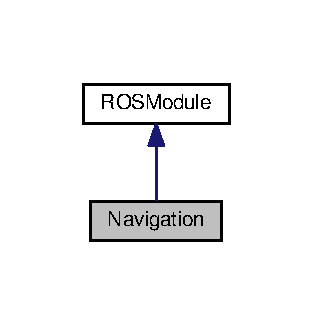
\includegraphics[width=150pt]{classNavigation__inherit__graph}
\end{center}
\end{figure}


Collaboration diagram for Navigation\+:
\nopagebreak
\begin{figure}[H]
\begin{center}
\leavevmode
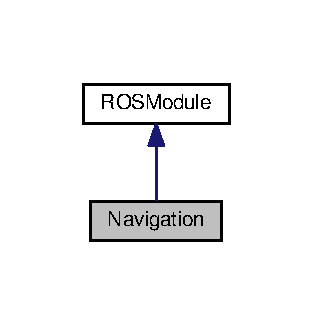
\includegraphics[width=150pt]{classNavigation__coll__graph}
\end{center}
\end{figure}
\subsection*{Public Member Functions}
\begin{DoxyCompactItemize}
\item 
bool \hyperlink{classNavigation_a31e234539cce5f116f23019246c01ff8}{move\+To\+Srv} (kids\+\_\+next\+\_\+door\+::move\+To\+::\+Request \&req, kids\+\_\+next\+\_\+door\+::move\+To\+::\+Response \&resp)
\begin{DoxyCompactList}\small\item\em Service server which gets new target pose in request and starts moving towards it. It returns true/false once the service call is completed. \end{DoxyCompactList}\item 
void \hyperlink{classNavigation_a6d6f40c4ccb483aea94d276907767dba}{initialize\+Service\+Servers} ()
\begin{DoxyCompactList}\small\item\em Method for initializinig service servers inherited from the \hyperlink{classROSModule}{R\+O\+S\+Module}. \end{DoxyCompactList}\item 
void \hyperlink{classNavigation_a94004249498512cba4b86a0933823584}{set\+Goal} (const geometry\+\_\+msgs\+::\+Pose\+Stamped \&goal\+Pose)
\begin{DoxyCompactList}\small\item\em Method to set new goal position. \end{DoxyCompactList}\item 
move\+\_\+base\+\_\+msgs\+::\+Move\+Base\+Goal \hyperlink{classNavigation_a03d605fee146a452bb91f9e6ae1af1b3}{get\+Goal} ()
\begin{DoxyCompactList}\small\item\em Method for accessing the private member goal\+Pose. \end{DoxyCompactList}\item 
\hyperlink{classNavigation_addd4022d716df48f4e55a1db69361ba7}{$\sim$\+Navigation} ()\hypertarget{classNavigation_addd4022d716df48f4e55a1db69361ba7}{}\label{classNavigation_addd4022d716df48f4e55a1db69361ba7}

\begin{DoxyCompactList}\small\item\em Default Destructor for navigation class. \end{DoxyCompactList}\end{DoxyCompactItemize}


\subsection{Member Function Documentation}
\index{Navigation@{Navigation}!get\+Goal@{get\+Goal}}
\index{get\+Goal@{get\+Goal}!Navigation@{Navigation}}
\subsubsection[{\texorpdfstring{get\+Goal()}{getGoal()}}]{\setlength{\rightskip}{0pt plus 5cm}move\+\_\+base\+\_\+msgs\+::\+Move\+Base\+Goal Navigation\+::get\+Goal (
\begin{DoxyParamCaption}
{}
\end{DoxyParamCaption}
)}\hypertarget{classNavigation_a03d605fee146a452bb91f9e6ae1af1b3}{}\label{classNavigation_a03d605fee146a452bb91f9e6ae1af1b3}


Method for accessing the private member goal\+Pose. 


\begin{DoxyParams}{Parameters}
{\em None} & \\
\hline
\end{DoxyParams}
\begin{DoxyReturn}{Returns}
move\+\_\+base\+\_\+msgs\+::\+Move\+Base\+Goal -\/ access to data member goal\+Pose 
\end{DoxyReturn}
\index{Navigation@{Navigation}!initialize\+Service\+Servers@{initialize\+Service\+Servers}}
\index{initialize\+Service\+Servers@{initialize\+Service\+Servers}!Navigation@{Navigation}}
\subsubsection[{\texorpdfstring{initialize\+Service\+Servers()}{initializeServiceServers()}}]{\setlength{\rightskip}{0pt plus 5cm}void Navigation\+::initialize\+Service\+Servers (
\begin{DoxyParamCaption}
{}
\end{DoxyParamCaption}
)\hspace{0.3cm}{\ttfamily [virtual]}}\hypertarget{classNavigation_a6d6f40c4ccb483aea94d276907767dba}{}\label{classNavigation_a6d6f40c4ccb483aea94d276907767dba}


Method for initializinig service servers inherited from the \hyperlink{classROSModule}{R\+O\+S\+Module}. 


\begin{DoxyParams}{Parameters}
{\em None} & \\
\hline
\end{DoxyParams}
\begin{DoxyReturn}{Returns}
None 
\end{DoxyReturn}


Reimplemented from \hyperlink{classROSModule_acdaf5d8d272814d30b9c15b9b20941ee}{R\+O\+S\+Module}.

\index{Navigation@{Navigation}!move\+To\+Srv@{move\+To\+Srv}}
\index{move\+To\+Srv@{move\+To\+Srv}!Navigation@{Navigation}}
\subsubsection[{\texorpdfstring{move\+To\+Srv(kids\+\_\+next\+\_\+door\+::move\+To\+::\+Request \&req, kids\+\_\+next\+\_\+door\+::move\+To\+::\+Response \&resp)}{moveToSrv(kids_next_door::moveTo::Request &req, kids_next_door::moveTo::Response &resp)}}]{\setlength{\rightskip}{0pt plus 5cm}bool Navigation\+::move\+To\+Srv (
\begin{DoxyParamCaption}
\item[{kids\+\_\+next\+\_\+door\+::move\+To\+::\+Request \&}]{req, }
\item[{kids\+\_\+next\+\_\+door\+::move\+To\+::\+Response \&}]{resp}
\end{DoxyParamCaption}
)}\hypertarget{classNavigation_a31e234539cce5f116f23019246c01ff8}{}\label{classNavigation_a31e234539cce5f116f23019246c01ff8}


Service server which gets new target pose in request and starts moving towards it. It returns true/false once the service call is completed. 


\begin{DoxyParams}{Parameters}
{\em req} & -\/ service request object of new target Pose \\
\hline
{\em resp} & -\/ service response object of completed action\\
\hline
\end{DoxyParams}
\begin{DoxyReturn}{Returns}
bool -\/ true when the service is completed 
\end{DoxyReturn}
\index{Navigation@{Navigation}!set\+Goal@{set\+Goal}}
\index{set\+Goal@{set\+Goal}!Navigation@{Navigation}}
\subsubsection[{\texorpdfstring{set\+Goal(const geometry\+\_\+msgs\+::\+Pose\+Stamped \&goal\+Pose)}{setGoal(const geometry_msgs::PoseStamped &goalPose)}}]{\setlength{\rightskip}{0pt plus 5cm}void Navigation\+::set\+Goal (
\begin{DoxyParamCaption}
\item[{const geometry\+\_\+msgs\+::\+Pose\+Stamped \&}]{goal\+Pose}
\end{DoxyParamCaption}
)}\hypertarget{classNavigation_a94004249498512cba4b86a0933823584}{}\label{classNavigation_a94004249498512cba4b86a0933823584}


Method to set new goal position. 


\begin{DoxyParams}{Parameters}
{\em goal\+Pose} & -\/ const reference to new goal position\\
\hline
\end{DoxyParams}
\begin{DoxyReturn}{Returns}
None 
\end{DoxyReturn}


The documentation for this class was generated from the following file\+:\begin{DoxyCompactItemize}
\item 
include/\hyperlink{Navigation_8hpp}{Navigation.\+hpp}\end{DoxyCompactItemize}

\hypertarget{classROSModule}{}\section{R\+O\+S\+Module Class Reference}
\label{classROSModule}\index{R\+O\+S\+Module@{R\+O\+S\+Module}}


Inheritance diagram for R\+O\+S\+Module\+:
\nopagebreak
\begin{figure}[H]
\begin{center}
\leavevmode
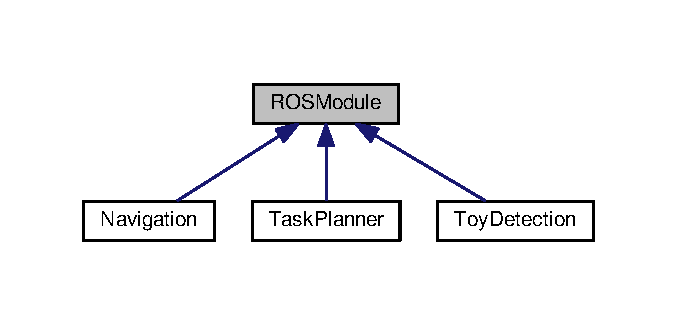
\includegraphics[width=325pt]{classROSModule__inherit__graph}
\end{center}
\end{figure}
\subsection*{Public Member Functions}
\begin{DoxyCompactItemize}
\item 
\hyperlink{classROSModule_a9efc72cd6ded210f0d140e03f6350ba2}{R\+O\+S\+Module} ()
\begin{DoxyCompactList}\small\item\em Constructor for class. \end{DoxyCompactList}\item 
virtual \hyperlink{classROSModule_afeaee6a49e898dbb1ad723270103a66e}{$\sim$\+R\+O\+S\+Module} ()
\begin{DoxyCompactList}\small\item\em Destructor for class. \end{DoxyCompactList}\item 
virtual void \hyperlink{classROSModule_a0e7a0518c74867505a4e8217c4413646}{initialize\+Subscribers} ()
\begin{DoxyCompactList}\small\item\em Function to initialize Subscribers for node. \end{DoxyCompactList}\item 
virtual void \hyperlink{classROSModule_afb506fedd0ac2412652618cd1e1d8e8e}{initialize\+Publishers} ()
\begin{DoxyCompactList}\small\item\em Function to initialize Publishers for node. \end{DoxyCompactList}\item 
virtual void \hyperlink{classROSModule_acdaf5d8d272814d30b9c15b9b20941ee}{initialize\+Service\+Servers} ()
\begin{DoxyCompactList}\small\item\em Function to initialize Service Servers for node. \end{DoxyCompactList}\item 
virtual void \hyperlink{classROSModule_a0155f960b33c0fb387ff5ef37fab743b}{initialize\+Service\+Clients} ()
\begin{DoxyCompactList}\small\item\em Function to initialize Service Clients for node. \end{DoxyCompactList}\item 
virtual void \hyperlink{classROSModule_a01c3d63aec5aeec426b16aacf2a0c756}{initialize\+Action\+Clients} ()
\begin{DoxyCompactList}\small\item\em Function to initialize Action Client for node. \end{DoxyCompactList}\item 
virtual void \hyperlink{classROSModule_a729d02696abb945a3bb34dbfe337ad77}{initialize\+Transform\+Broadcaster} ()
\begin{DoxyCompactList}\small\item\em Function to initialize Transform Broadcasters for node. \end{DoxyCompactList}\item 
virtual void \hyperlink{classROSModule_a0efdf08daec048431fdbcf20d65b6606}{initialize\+Transform\+Listener} ()
\begin{DoxyCompactList}\small\item\em Function to initialize Transform Listener for node. \end{DoxyCompactList}\end{DoxyCompactItemize}


\subsection{Constructor \& Destructor Documentation}
\index{R\+O\+S\+Module@{R\+O\+S\+Module}!R\+O\+S\+Module@{R\+O\+S\+Module}}
\index{R\+O\+S\+Module@{R\+O\+S\+Module}!R\+O\+S\+Module@{R\+O\+S\+Module}}
\subsubsection[{\texorpdfstring{R\+O\+S\+Module()}{ROSModule()}}]{\setlength{\rightskip}{0pt plus 5cm}R\+O\+S\+Module\+::\+R\+O\+S\+Module (
\begin{DoxyParamCaption}
{}
\end{DoxyParamCaption}
)\hspace{0.3cm}{\ttfamily [inline]}}\hypertarget{classROSModule_a9efc72cd6ded210f0d140e03f6350ba2}{}\label{classROSModule_a9efc72cd6ded210f0d140e03f6350ba2}


Constructor for class. 


\begin{DoxyParams}{Parameters}
{\em None} & \\
\hline
\end{DoxyParams}
\begin{DoxyReturn}{Returns}
None 
\end{DoxyReturn}
\index{R\+O\+S\+Module@{R\+O\+S\+Module}!````~R\+O\+S\+Module@{$\sim$\+R\+O\+S\+Module}}
\index{````~R\+O\+S\+Module@{$\sim$\+R\+O\+S\+Module}!R\+O\+S\+Module@{R\+O\+S\+Module}}
\subsubsection[{\texorpdfstring{$\sim$\+R\+O\+S\+Module()}{~ROSModule()}}]{\setlength{\rightskip}{0pt plus 5cm}virtual R\+O\+S\+Module\+::$\sim$\+R\+O\+S\+Module (
\begin{DoxyParamCaption}
{}
\end{DoxyParamCaption}
)\hspace{0.3cm}{\ttfamily [inline]}, {\ttfamily [virtual]}}\hypertarget{classROSModule_afeaee6a49e898dbb1ad723270103a66e}{}\label{classROSModule_afeaee6a49e898dbb1ad723270103a66e}


Destructor for class. 


\begin{DoxyParams}{Parameters}
{\em None} & \\
\hline
\end{DoxyParams}
\begin{DoxyReturn}{Returns}
None 
\end{DoxyReturn}


\subsection{Member Function Documentation}
\index{R\+O\+S\+Module@{R\+O\+S\+Module}!initialize\+Action\+Clients@{initialize\+Action\+Clients}}
\index{initialize\+Action\+Clients@{initialize\+Action\+Clients}!R\+O\+S\+Module@{R\+O\+S\+Module}}
\subsubsection[{\texorpdfstring{initialize\+Action\+Clients()}{initializeActionClients()}}]{\setlength{\rightskip}{0pt plus 5cm}virtual void R\+O\+S\+Module\+::initialize\+Action\+Clients (
\begin{DoxyParamCaption}
{}
\end{DoxyParamCaption}
)\hspace{0.3cm}{\ttfamily [inline]}, {\ttfamily [virtual]}}\hypertarget{classROSModule_a01c3d63aec5aeec426b16aacf2a0c756}{}\label{classROSModule_a01c3d63aec5aeec426b16aacf2a0c756}


Function to initialize Action Client for node. 


\begin{DoxyParams}{Parameters}
{\em None} & \\
\hline
\end{DoxyParams}
\begin{DoxyReturn}{Returns}
None 
\end{DoxyReturn}
\index{R\+O\+S\+Module@{R\+O\+S\+Module}!initialize\+Publishers@{initialize\+Publishers}}
\index{initialize\+Publishers@{initialize\+Publishers}!R\+O\+S\+Module@{R\+O\+S\+Module}}
\subsubsection[{\texorpdfstring{initialize\+Publishers()}{initializePublishers()}}]{\setlength{\rightskip}{0pt plus 5cm}virtual void R\+O\+S\+Module\+::initialize\+Publishers (
\begin{DoxyParamCaption}
{}
\end{DoxyParamCaption}
)\hspace{0.3cm}{\ttfamily [inline]}, {\ttfamily [virtual]}}\hypertarget{classROSModule_afb506fedd0ac2412652618cd1e1d8e8e}{}\label{classROSModule_afb506fedd0ac2412652618cd1e1d8e8e}


Function to initialize Publishers for node. 


\begin{DoxyParams}{Parameters}
{\em None} & \\
\hline
\end{DoxyParams}
\begin{DoxyReturn}{Returns}
None 
\end{DoxyReturn}
\index{R\+O\+S\+Module@{R\+O\+S\+Module}!initialize\+Service\+Clients@{initialize\+Service\+Clients}}
\index{initialize\+Service\+Clients@{initialize\+Service\+Clients}!R\+O\+S\+Module@{R\+O\+S\+Module}}
\subsubsection[{\texorpdfstring{initialize\+Service\+Clients()}{initializeServiceClients()}}]{\setlength{\rightskip}{0pt plus 5cm}virtual void R\+O\+S\+Module\+::initialize\+Service\+Clients (
\begin{DoxyParamCaption}
{}
\end{DoxyParamCaption}
)\hspace{0.3cm}{\ttfamily [inline]}, {\ttfamily [virtual]}}\hypertarget{classROSModule_a0155f960b33c0fb387ff5ef37fab743b}{}\label{classROSModule_a0155f960b33c0fb387ff5ef37fab743b}


Function to initialize Service Clients for node. 


\begin{DoxyParams}{Parameters}
{\em None} & \\
\hline
\end{DoxyParams}
\begin{DoxyReturn}{Returns}
None 
\end{DoxyReturn}


Reimplemented in \hyperlink{classTaskPlanner_a6347f18c5b24392c58d4ff87ff7f256c}{Task\+Planner}.

\index{R\+O\+S\+Module@{R\+O\+S\+Module}!initialize\+Service\+Servers@{initialize\+Service\+Servers}}
\index{initialize\+Service\+Servers@{initialize\+Service\+Servers}!R\+O\+S\+Module@{R\+O\+S\+Module}}
\subsubsection[{\texorpdfstring{initialize\+Service\+Servers()}{initializeServiceServers()}}]{\setlength{\rightskip}{0pt plus 5cm}virtual void R\+O\+S\+Module\+::initialize\+Service\+Servers (
\begin{DoxyParamCaption}
{}
\end{DoxyParamCaption}
)\hspace{0.3cm}{\ttfamily [inline]}, {\ttfamily [virtual]}}\hypertarget{classROSModule_acdaf5d8d272814d30b9c15b9b20941ee}{}\label{classROSModule_acdaf5d8d272814d30b9c15b9b20941ee}


Function to initialize Service Servers for node. 


\begin{DoxyParams}{Parameters}
{\em None} & \\
\hline
\end{DoxyParams}
\begin{DoxyReturn}{Returns}
None 
\end{DoxyReturn}


Reimplemented in \hyperlink{classNavigation_a6d6f40c4ccb483aea94d276907767dba}{Navigation}, and \hyperlink{classToyDetection_a410f48815e4e1727c73d41013fc9a7f3}{Toy\+Detection}.

\index{R\+O\+S\+Module@{R\+O\+S\+Module}!initialize\+Subscribers@{initialize\+Subscribers}}
\index{initialize\+Subscribers@{initialize\+Subscribers}!R\+O\+S\+Module@{R\+O\+S\+Module}}
\subsubsection[{\texorpdfstring{initialize\+Subscribers()}{initializeSubscribers()}}]{\setlength{\rightskip}{0pt plus 5cm}virtual void R\+O\+S\+Module\+::initialize\+Subscribers (
\begin{DoxyParamCaption}
{}
\end{DoxyParamCaption}
)\hspace{0.3cm}{\ttfamily [inline]}, {\ttfamily [virtual]}}\hypertarget{classROSModule_a0e7a0518c74867505a4e8217c4413646}{}\label{classROSModule_a0e7a0518c74867505a4e8217c4413646}


Function to initialize Subscribers for node. 


\begin{DoxyParams}{Parameters}
{\em None} & \\
\hline
\end{DoxyParams}
\begin{DoxyReturn}{Returns}
None 
\end{DoxyReturn}


Reimplemented in \hyperlink{classToyDetection_a0bc77c348ab5675c6ee59e9d184e483f}{Toy\+Detection}.

\index{R\+O\+S\+Module@{R\+O\+S\+Module}!initialize\+Transform\+Broadcaster@{initialize\+Transform\+Broadcaster}}
\index{initialize\+Transform\+Broadcaster@{initialize\+Transform\+Broadcaster}!R\+O\+S\+Module@{R\+O\+S\+Module}}
\subsubsection[{\texorpdfstring{initialize\+Transform\+Broadcaster()}{initializeTransformBroadcaster()}}]{\setlength{\rightskip}{0pt plus 5cm}virtual void R\+O\+S\+Module\+::initialize\+Transform\+Broadcaster (
\begin{DoxyParamCaption}
{}
\end{DoxyParamCaption}
)\hspace{0.3cm}{\ttfamily [inline]}, {\ttfamily [virtual]}}\hypertarget{classROSModule_a729d02696abb945a3bb34dbfe337ad77}{}\label{classROSModule_a729d02696abb945a3bb34dbfe337ad77}


Function to initialize Transform Broadcasters for node. 


\begin{DoxyParams}{Parameters}
{\em None} & \\
\hline
\end{DoxyParams}
\begin{DoxyReturn}{Returns}
None 
\end{DoxyReturn}
\index{R\+O\+S\+Module@{R\+O\+S\+Module}!initialize\+Transform\+Listener@{initialize\+Transform\+Listener}}
\index{initialize\+Transform\+Listener@{initialize\+Transform\+Listener}!R\+O\+S\+Module@{R\+O\+S\+Module}}
\subsubsection[{\texorpdfstring{initialize\+Transform\+Listener()}{initializeTransformListener()}}]{\setlength{\rightskip}{0pt plus 5cm}virtual void R\+O\+S\+Module\+::initialize\+Transform\+Listener (
\begin{DoxyParamCaption}
{}
\end{DoxyParamCaption}
)\hspace{0.3cm}{\ttfamily [inline]}, {\ttfamily [virtual]}}\hypertarget{classROSModule_a0efdf08daec048431fdbcf20d65b6606}{}\label{classROSModule_a0efdf08daec048431fdbcf20d65b6606}


Function to initialize Transform Listener for node. 


\begin{DoxyParams}{Parameters}
{\em None} & \\
\hline
\end{DoxyParams}
\begin{DoxyReturn}{Returns}
None 
\end{DoxyReturn}


The documentation for this class was generated from the following file\+:\begin{DoxyCompactItemize}
\item 
include/\hyperlink{ROSModule_8hpp}{R\+O\+S\+Module.\+hpp}\end{DoxyCompactItemize}

\hypertarget{classTaskPlanner}{}\section{Task\+Planner Class Reference}
\label{classTaskPlanner}\index{Task\+Planner@{Task\+Planner}}


Inheritance diagram for Task\+Planner\+:
\nopagebreak
\begin{figure}[H]
\begin{center}
\leavevmode
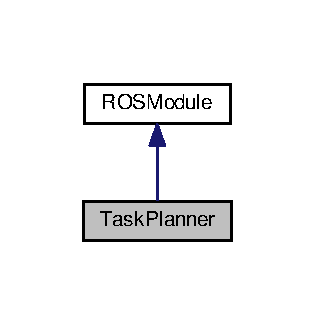
\includegraphics[width=151pt]{classTaskPlanner__inherit__graph}
\end{center}
\end{figure}


Collaboration diagram for Task\+Planner\+:
\nopagebreak
\begin{figure}[H]
\begin{center}
\leavevmode
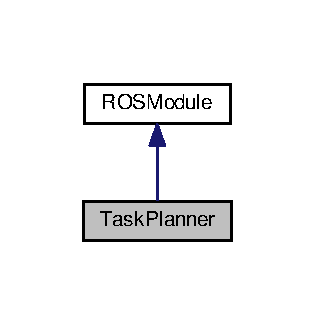
\includegraphics[width=151pt]{classTaskPlanner__coll__graph}
\end{center}
\end{figure}
\subsection*{Public Member Functions}
\begin{DoxyCompactItemize}
\item 
\hyperlink{classTaskPlanner_a63d11be6cf3d676ef3256ab4019537b7}{Task\+Planner} ()
\begin{DoxyCompactList}\small\item\em Constructor for class. \end{DoxyCompactList}\item 
\hyperlink{classTaskPlanner_a39b6eab2a22f8249d046330e833571df}{Task\+Planner} (std\+::istream \&input\+Stream, std\+::ostream \&output\+Stream)
\begin{DoxyCompactList}\small\item\em Constructor for class with input/output stream arguments. \end{DoxyCompactList}\item 
\hyperlink{classTaskPlanner_a551378501f7a1e6304c207c25b2400db}{$\sim$\+Task\+Planner} ()
\begin{DoxyCompactList}\small\item\em Destructor for class. \end{DoxyCompactList}\item 
void \hyperlink{classTaskPlanner_a6347f18c5b24392c58d4ff87ff7f256c}{initialize\+Service\+Clients} ()
\begin{DoxyCompactList}\small\item\em Function to initialize Service Clients. \end{DoxyCompactList}\item 
int \hyperlink{classTaskPlanner_a0a9c473acb9493472dca65bb9e17eede}{move\+To\+Pose} (geometry\+\_\+msgs\+::\+Pose\+Stamped pose)
\begin{DoxyCompactList}\small\item\em Calls service to move Tiago Base to given position. \end{DoxyCompactList}\item 
int \hyperlink{classTaskPlanner_aa2522c94c2269b1abbf8a811b5a98456}{look\+For\+Toy} (int toy\+ID)
\begin{DoxyCompactList}\small\item\em Calls service to look for Ar\+Uco markers on toys. \end{DoxyCompactList}\item 
int \hyperlink{classTaskPlanner_ab618ec1d38428184f939b0a661068ea5}{go\+To\+Toy} ()
\begin{DoxyCompactList}\small\item\em Calls service to move Tiago Base to Toy position. \end{DoxyCompactList}\item 
int \hyperlink{classTaskPlanner_a8c564e25fffe19f9164723fb8dac03a2}{go\+To\+Storage} ()
\begin{DoxyCompactList}\small\item\em Calls service to move Tiago to Toy Storage Location. \end{DoxyCompactList}\item 
int \hyperlink{classTaskPlanner_abb44ac3329ee21a3da250492c564ab74}{search} (geometry\+\_\+msgs\+::\+Pose\+Stamped search\+Pose)
\begin{DoxyCompactList}\small\item\em search operation for scanning the area for Ar\+Uco markers \end{DoxyCompactList}\item 
int \hyperlink{classTaskPlanner_a3b20363d2cb4b2abe5af5646c76b85d5}{pick\+Up\+Toy} ()
\begin{DoxyCompactList}\small\item\em Calls service to pickup Toy. \end{DoxyCompactList}\item 
int \hyperlink{classTaskPlanner_acc35c29d80d8849cfd73070633eaa3e1}{store\+Toy} ()
\begin{DoxyCompactList}\small\item\em Calls service to store toy in storage. \end{DoxyCompactList}\item 
void \hyperlink{classTaskPlanner_a9a7f370e15d723831153992c6b6f9cd7}{shutdown\+Robot} ()
\begin{DoxyCompactList}\small\item\em Shuts down R\+OS nodes. \end{DoxyCompactList}\item 
int \hyperlink{classTaskPlanner_ae0d072f084358dcda2ff6fee665aad35}{task\+Planner} ()
\begin{DoxyCompactList}\small\item\em Main method which switches from the current task to the next one based on feedback from the robot. \end{DoxyCompactList}\end{DoxyCompactItemize}


\subsection{Constructor \& Destructor Documentation}
\index{Task\+Planner@{Task\+Planner}!Task\+Planner@{Task\+Planner}}
\index{Task\+Planner@{Task\+Planner}!Task\+Planner@{Task\+Planner}}
\subsubsection[{\texorpdfstring{Task\+Planner()}{TaskPlanner()}}]{\setlength{\rightskip}{0pt plus 5cm}Task\+Planner\+::\+Task\+Planner (
\begin{DoxyParamCaption}
{}
\end{DoxyParamCaption}
)}\hypertarget{classTaskPlanner_a63d11be6cf3d676ef3256ab4019537b7}{}\label{classTaskPlanner_a63d11be6cf3d676ef3256ab4019537b7}


Constructor for class. 


\begin{DoxyParams}{Parameters}
{\em None} & \\
\hline
\end{DoxyParams}
\begin{DoxyReturn}{Returns}
None 
\end{DoxyReturn}
\index{Task\+Planner@{Task\+Planner}!Task\+Planner@{Task\+Planner}}
\index{Task\+Planner@{Task\+Planner}!Task\+Planner@{Task\+Planner}}
\subsubsection[{\texorpdfstring{Task\+Planner(std\+::istream \&input\+Stream, std\+::ostream \&output\+Stream)}{TaskPlanner(std::istream &inputStream, std::ostream &outputStream)}}]{\setlength{\rightskip}{0pt plus 5cm}Task\+Planner\+::\+Task\+Planner (
\begin{DoxyParamCaption}
\item[{std\+::istream \&}]{input\+Stream, }
\item[{std\+::ostream \&}]{output\+Stream}
\end{DoxyParamCaption}
)}\hypertarget{classTaskPlanner_a39b6eab2a22f8249d046330e833571df}{}\label{classTaskPlanner_a39b6eab2a22f8249d046330e833571df}


Constructor for class with input/output stream arguments. 


\begin{DoxyParams}{Parameters}
{\em input\+Stream} & Input Stream object\\
\hline
{\em output\+Stream} & Output Stream object\\
\hline
\end{DoxyParams}
\begin{DoxyReturn}{Returns}
None 
\end{DoxyReturn}
\index{Task\+Planner@{Task\+Planner}!````~Task\+Planner@{$\sim$\+Task\+Planner}}
\index{````~Task\+Planner@{$\sim$\+Task\+Planner}!Task\+Planner@{Task\+Planner}}
\subsubsection[{\texorpdfstring{$\sim$\+Task\+Planner()}{~TaskPlanner()}}]{\setlength{\rightskip}{0pt plus 5cm}Task\+Planner\+::$\sim$\+Task\+Planner (
\begin{DoxyParamCaption}
{}
\end{DoxyParamCaption}
)}\hypertarget{classTaskPlanner_a551378501f7a1e6304c207c25b2400db}{}\label{classTaskPlanner_a551378501f7a1e6304c207c25b2400db}


Destructor for class. 


\begin{DoxyParams}{Parameters}
{\em None} & \\
\hline
\end{DoxyParams}
\begin{DoxyReturn}{Returns}
None 
\end{DoxyReturn}


\subsection{Member Function Documentation}
\index{Task\+Planner@{Task\+Planner}!go\+To\+Storage@{go\+To\+Storage}}
\index{go\+To\+Storage@{go\+To\+Storage}!Task\+Planner@{Task\+Planner}}
\subsubsection[{\texorpdfstring{go\+To\+Storage()}{goToStorage()}}]{\setlength{\rightskip}{0pt plus 5cm}int Task\+Planner\+::go\+To\+Storage (
\begin{DoxyParamCaption}
{}
\end{DoxyParamCaption}
)}\hypertarget{classTaskPlanner_a8c564e25fffe19f9164723fb8dac03a2}{}\label{classTaskPlanner_a8c564e25fffe19f9164723fb8dac03a2}


Calls service to move Tiago to Toy Storage Location. 


\begin{DoxyParams}{Parameters}
{\em None} & \\
\hline
\end{DoxyParams}
\begin{DoxyReturn}{Returns}
Int with function execution status. -\/1 for call failure, 0 when call is successful but storage not reachable, 1 when storage is reached 
\end{DoxyReturn}
\index{Task\+Planner@{Task\+Planner}!go\+To\+Toy@{go\+To\+Toy}}
\index{go\+To\+Toy@{go\+To\+Toy}!Task\+Planner@{Task\+Planner}}
\subsubsection[{\texorpdfstring{go\+To\+Toy()}{goToToy()}}]{\setlength{\rightskip}{0pt plus 5cm}int Task\+Planner\+::go\+To\+Toy (
\begin{DoxyParamCaption}
{}
\end{DoxyParamCaption}
)}\hypertarget{classTaskPlanner_ab618ec1d38428184f939b0a661068ea5}{}\label{classTaskPlanner_ab618ec1d38428184f939b0a661068ea5}


Calls service to move Tiago Base to Toy position. 


\begin{DoxyParams}{Parameters}
{\em None} & \\
\hline
\end{DoxyParams}
\begin{DoxyReturn}{Returns}
Int with function execution status. -\/1 for call failure, 0 when call is successful but position not reachable, 1 when position is reached 
\end{DoxyReturn}
\index{Task\+Planner@{Task\+Planner}!initialize\+Service\+Clients@{initialize\+Service\+Clients}}
\index{initialize\+Service\+Clients@{initialize\+Service\+Clients}!Task\+Planner@{Task\+Planner}}
\subsubsection[{\texorpdfstring{initialize\+Service\+Clients()}{initializeServiceClients()}}]{\setlength{\rightskip}{0pt plus 5cm}void Task\+Planner\+::initialize\+Service\+Clients (
\begin{DoxyParamCaption}
{}
\end{DoxyParamCaption}
)\hspace{0.3cm}{\ttfamily [virtual]}}\hypertarget{classTaskPlanner_a6347f18c5b24392c58d4ff87ff7f256c}{}\label{classTaskPlanner_a6347f18c5b24392c58d4ff87ff7f256c}


Function to initialize Service Clients. 


\begin{DoxyParams}{Parameters}
{\em None} & \\
\hline
\end{DoxyParams}
\begin{DoxyReturn}{Returns}
None 
\end{DoxyReturn}


Reimplemented from \hyperlink{classROSModule_a0155f960b33c0fb387ff5ef37fab743b}{R\+O\+S\+Module}.

\index{Task\+Planner@{Task\+Planner}!look\+For\+Toy@{look\+For\+Toy}}
\index{look\+For\+Toy@{look\+For\+Toy}!Task\+Planner@{Task\+Planner}}
\subsubsection[{\texorpdfstring{look\+For\+Toy(int toy\+I\+D)}{lookForToy(int toyID)}}]{\setlength{\rightskip}{0pt plus 5cm}int Task\+Planner\+::look\+For\+Toy (
\begin{DoxyParamCaption}
\item[{int}]{toy\+ID}
\end{DoxyParamCaption}
)}\hypertarget{classTaskPlanner_aa2522c94c2269b1abbf8a811b5a98456}{}\label{classTaskPlanner_aa2522c94c2269b1abbf8a811b5a98456}


Calls service to look for Ar\+Uco markers on toys. 


\begin{DoxyParams}{Parameters}
{\em toy\+ID} & ID of the Ar\+Uco marker to be searched\\
\hline
\end{DoxyParams}
\begin{DoxyReturn}{Returns}
Int with function execution status. -\/1 for call failure, 0 when call is successful but toy not visible, 1 when toy visible 
\end{DoxyReturn}
\index{Task\+Planner@{Task\+Planner}!move\+To\+Pose@{move\+To\+Pose}}
\index{move\+To\+Pose@{move\+To\+Pose}!Task\+Planner@{Task\+Planner}}
\subsubsection[{\texorpdfstring{move\+To\+Pose(geometry\+\_\+msgs\+::\+Pose\+Stamped pose)}{moveToPose(geometry_msgs::PoseStamped pose)}}]{\setlength{\rightskip}{0pt plus 5cm}int Task\+Planner\+::move\+To\+Pose (
\begin{DoxyParamCaption}
\item[{geometry\+\_\+msgs\+::\+Pose\+Stamped}]{pose}
\end{DoxyParamCaption}
)}\hypertarget{classTaskPlanner_a0a9c473acb9493472dca65bb9e17eede}{}\label{classTaskPlanner_a0a9c473acb9493472dca65bb9e17eede}


Calls service to move Tiago Base to given position. 


\begin{DoxyParams}{Parameters}
{\em pose} & The goal position robot is to be moved to\\
\hline
\end{DoxyParams}
\begin{DoxyReturn}{Returns}
Int with function execution status. -\/1 for call failure, 0 when call is successful but position not reachable, 1 when position is reached 
\end{DoxyReturn}
\index{Task\+Planner@{Task\+Planner}!pick\+Up\+Toy@{pick\+Up\+Toy}}
\index{pick\+Up\+Toy@{pick\+Up\+Toy}!Task\+Planner@{Task\+Planner}}
\subsubsection[{\texorpdfstring{pick\+Up\+Toy()}{pickUpToy()}}]{\setlength{\rightskip}{0pt plus 5cm}int Task\+Planner\+::pick\+Up\+Toy (
\begin{DoxyParamCaption}
{}
\end{DoxyParamCaption}
)}\hypertarget{classTaskPlanner_a3b20363d2cb4b2abe5af5646c76b85d5}{}\label{classTaskPlanner_a3b20363d2cb4b2abe5af5646c76b85d5}


Calls service to pickup Toy. 


\begin{DoxyParams}{Parameters}
{\em None} & \\
\hline
\end{DoxyParams}
\begin{DoxyReturn}{Returns}
Int with function execution status. -\/1 for call failure, 0 when call is successful but toy could not be picked up, 1 when toy is successfully picked up 
\end{DoxyReturn}
\index{Task\+Planner@{Task\+Planner}!search@{search}}
\index{search@{search}!Task\+Planner@{Task\+Planner}}
\subsubsection[{\texorpdfstring{search(geometry\+\_\+msgs\+::\+Pose\+Stamped search\+Pose)}{search(geometry_msgs::PoseStamped searchPose)}}]{\setlength{\rightskip}{0pt plus 5cm}int Task\+Planner\+::search (
\begin{DoxyParamCaption}
\item[{geometry\+\_\+msgs\+::\+Pose\+Stamped}]{search\+Pose}
\end{DoxyParamCaption}
)}\hypertarget{classTaskPlanner_abb44ac3329ee21a3da250492c564ab74}{}\label{classTaskPlanner_abb44ac3329ee21a3da250492c564ab74}


search operation for scanning the area for Ar\+Uco markers 


\begin{DoxyParams}{Parameters}
{\em search\+Pose} & Pose of the next location to go to loook for toy\\
\hline
\end{DoxyParams}
\begin{DoxyReturn}{Returns}
Int with function execution status. -\/1 for call failure, 0 when call is successful but position not reachable, 1 when position is reached 
\end{DoxyReturn}
\index{Task\+Planner@{Task\+Planner}!shutdown\+Robot@{shutdown\+Robot}}
\index{shutdown\+Robot@{shutdown\+Robot}!Task\+Planner@{Task\+Planner}}
\subsubsection[{\texorpdfstring{shutdown\+Robot()}{shutdownRobot()}}]{\setlength{\rightskip}{0pt plus 5cm}void Task\+Planner\+::shutdown\+Robot (
\begin{DoxyParamCaption}
{}
\end{DoxyParamCaption}
)}\hypertarget{classTaskPlanner_a9a7f370e15d723831153992c6b6f9cd7}{}\label{classTaskPlanner_a9a7f370e15d723831153992c6b6f9cd7}


Shuts down R\+OS nodes. 


\begin{DoxyParams}{Parameters}
{\em None} & \\
\hline
\end{DoxyParams}
\begin{DoxyReturn}{Returns}
None 
\end{DoxyReturn}
\index{Task\+Planner@{Task\+Planner}!store\+Toy@{store\+Toy}}
\index{store\+Toy@{store\+Toy}!Task\+Planner@{Task\+Planner}}
\subsubsection[{\texorpdfstring{store\+Toy()}{storeToy()}}]{\setlength{\rightskip}{0pt plus 5cm}int Task\+Planner\+::store\+Toy (
\begin{DoxyParamCaption}
{}
\end{DoxyParamCaption}
)}\hypertarget{classTaskPlanner_acc35c29d80d8849cfd73070633eaa3e1}{}\label{classTaskPlanner_acc35c29d80d8849cfd73070633eaa3e1}


Calls service to store toy in storage. 


\begin{DoxyParams}{Parameters}
{\em None} & \\
\hline
\end{DoxyParams}
\begin{DoxyReturn}{Returns}
Int with function execution status. -\/1 for call failure, 0 when call is successful but toy could not be placed, 1 when toy is successfully placed in storage 
\end{DoxyReturn}
\index{Task\+Planner@{Task\+Planner}!task\+Planner@{task\+Planner}}
\index{task\+Planner@{task\+Planner}!Task\+Planner@{Task\+Planner}}
\subsubsection[{\texorpdfstring{task\+Planner()}{taskPlanner()}}]{\setlength{\rightskip}{0pt plus 5cm}int Task\+Planner\+::task\+Planner (
\begin{DoxyParamCaption}
{}
\end{DoxyParamCaption}
)}\hypertarget{classTaskPlanner_ae0d072f084358dcda2ff6fee665aad35}{}\label{classTaskPlanner_ae0d072f084358dcda2ff6fee665aad35}


Main method which switches from the current task to the next one based on feedback from the robot. 


\begin{DoxyParams}{Parameters}
{\em None} & \\
\hline
\end{DoxyParams}
\begin{DoxyReturn}{Returns}
None 
\end{DoxyReturn}


The documentation for this class was generated from the following file\+:\begin{DoxyCompactItemize}
\item 
include/\hyperlink{TaskPlanner_8hpp}{Task\+Planner.\+hpp}\end{DoxyCompactItemize}

\hypertarget{classToyDetection}{}\section{Toy\+Detection Class Reference}
\label{classToyDetection}\index{Toy\+Detection@{Toy\+Detection}}


Inheritance diagram for Toy\+Detection\+:
\nopagebreak
\begin{figure}[H]
\begin{center}
\leavevmode
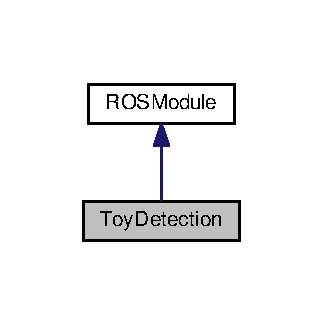
\includegraphics[width=155pt]{classToyDetection__inherit__graph}
\end{center}
\end{figure}


Collaboration diagram for Toy\+Detection\+:
\nopagebreak
\begin{figure}[H]
\begin{center}
\leavevmode
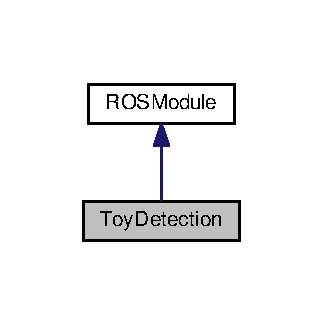
\includegraphics[width=155pt]{classToyDetection__coll__graph}
\end{center}
\end{figure}
\subsection*{Public Member Functions}
\begin{DoxyCompactItemize}
\item 
\hyperlink{classToyDetection_ae10edf712502b78e3b49e0421c877ea1}{Toy\+Detection} ()\hypertarget{classToyDetection_ae10edf712502b78e3b49e0421c877ea1}{}\label{classToyDetection_ae10edf712502b78e3b49e0421c877ea1}

\begin{DoxyCompactList}\small\item\em Default Constructor. \end{DoxyCompactList}\item 
void \hyperlink{classToyDetection_a0bc77c348ab5675c6ee59e9d184e483f}{initialize\+Subscribers} ()
\begin{DoxyCompactList}\small\item\em Method to initialize Subscribers, inherited from \hyperlink{classROSModule}{R\+O\+S\+Module}. \end{DoxyCompactList}\item 
void \hyperlink{classToyDetection_a410f48815e4e1727c73d41013fc9a7f3}{initialize\+Service\+Servers} ()
\begin{DoxyCompactList}\small\item\em Method to initialize Service Servers, inherited from \hyperlink{classROSModule}{R\+O\+S\+Module}. \end{DoxyCompactList}\item 
int \hyperlink{classToyDetection_a7198404077e6a5e5a3bb9b438b95b111}{detect\+Ar\+Uco} ()
\begin{DoxyCompactList}\small\item\em Method to check of Ar\+Uco is detected and storing the pose by calling the /knd/found\+Toy service. \end{DoxyCompactList}\item 
void \hyperlink{classToyDetection_a8a59388c998beaa5b2a2d4f4c6f5f63d}{detection\+Cb} (const std\+\_\+msgs\+::\+Bool\+::\+Const\+Ptr \&detection\+Flag)
\begin{DoxyCompactList}\small\item\em Callback method for detection flag. \end{DoxyCompactList}\item 
bool \hyperlink{classToyDetection_a124390e2ea87d3051e403caf738a9168}{find\+Toy\+Srv} (kids\+\_\+next\+\_\+door\+::toy\+Found\+::\+Request \&req, kids\+\_\+next\+\_\+door\+::toy\+Found\+::\+Response \&resp)
\begin{DoxyCompactList}\small\item\em R\+OS serice to check and return goal Pose if toy is found. \end{DoxyCompactList}\end{DoxyCompactItemize}


\subsection{Member Function Documentation}
\index{Toy\+Detection@{Toy\+Detection}!detect\+Ar\+Uco@{detect\+Ar\+Uco}}
\index{detect\+Ar\+Uco@{detect\+Ar\+Uco}!Toy\+Detection@{Toy\+Detection}}
\subsubsection[{\texorpdfstring{detect\+Ar\+Uco()}{detectArUco()}}]{\setlength{\rightskip}{0pt plus 5cm}int Toy\+Detection\+::detect\+Ar\+Uco (
\begin{DoxyParamCaption}
{}
\end{DoxyParamCaption}
)}\hypertarget{classToyDetection_a7198404077e6a5e5a3bb9b438b95b111}{}\label{classToyDetection_a7198404077e6a5e5a3bb9b438b95b111}


Method to check of Ar\+Uco is detected and storing the pose by calling the /knd/found\+Toy service. 


\begin{DoxyParams}{Parameters}
{\em None} & \\
\hline
\end{DoxyParams}
\begin{DoxyReturn}{Returns}
int -\/ 1 if Ar\+Uco is detected 0 otherwise 
\end{DoxyReturn}
\index{Toy\+Detection@{Toy\+Detection}!detection\+Cb@{detection\+Cb}}
\index{detection\+Cb@{detection\+Cb}!Toy\+Detection@{Toy\+Detection}}
\subsubsection[{\texorpdfstring{detection\+Cb(const std\+\_\+msgs\+::\+Bool\+::\+Const\+Ptr \&detection\+Flag)}{detectionCb(const std_msgs::Bool::ConstPtr &detectionFlag)}}]{\setlength{\rightskip}{0pt plus 5cm}void Toy\+Detection\+::detection\+Cb (
\begin{DoxyParamCaption}
\item[{const std\+\_\+msgs\+::\+Bool\+::\+Const\+Ptr \&}]{detection\+Flag}
\end{DoxyParamCaption}
)}\hypertarget{classToyDetection_a8a59388c998beaa5b2a2d4f4c6f5f63d}{}\label{classToyDetection_a8a59388c998beaa5b2a2d4f4c6f5f63d}


Callback method for detection flag. 


\begin{DoxyParams}{Parameters}
{\em detection\+Flag} & -\/ const reference to a detection flag bool \\
\hline
\end{DoxyParams}
\begin{DoxyReturn}{Returns}
None 
\end{DoxyReturn}
\index{Toy\+Detection@{Toy\+Detection}!find\+Toy\+Srv@{find\+Toy\+Srv}}
\index{find\+Toy\+Srv@{find\+Toy\+Srv}!Toy\+Detection@{Toy\+Detection}}
\subsubsection[{\texorpdfstring{find\+Toy\+Srv(kids\+\_\+next\+\_\+door\+::toy\+Found\+::\+Request \&req, kids\+\_\+next\+\_\+door\+::toy\+Found\+::\+Response \&resp)}{findToySrv(kids_next_door::toyFound::Request &req, kids_next_door::toyFound::Response &resp)}}]{\setlength{\rightskip}{0pt plus 5cm}bool Toy\+Detection\+::find\+Toy\+Srv (
\begin{DoxyParamCaption}
\item[{kids\+\_\+next\+\_\+door\+::toy\+Found\+::\+Request \&}]{req, }
\item[{kids\+\_\+next\+\_\+door\+::toy\+Found\+::\+Response \&}]{resp}
\end{DoxyParamCaption}
)}\hypertarget{classToyDetection_a124390e2ea87d3051e403caf738a9168}{}\label{classToyDetection_a124390e2ea87d3051e403caf738a9168}


R\+OS serice to check and return goal Pose if toy is found. 


\begin{DoxyParams}{Parameters}
{\em req} & -\/ service request uses integer id for a tag \\
\hline
{\em resp} & -\/ service response object contains bool for detection and geometry\+\_\+msgs\+::\+Pose\+Stamped msg for target Pose \\
\hline
\end{DoxyParams}
\index{Toy\+Detection@{Toy\+Detection}!initialize\+Service\+Servers@{initialize\+Service\+Servers}}
\index{initialize\+Service\+Servers@{initialize\+Service\+Servers}!Toy\+Detection@{Toy\+Detection}}
\subsubsection[{\texorpdfstring{initialize\+Service\+Servers()}{initializeServiceServers()}}]{\setlength{\rightskip}{0pt plus 5cm}void Toy\+Detection\+::initialize\+Service\+Servers (
\begin{DoxyParamCaption}
{}
\end{DoxyParamCaption}
)\hspace{0.3cm}{\ttfamily [virtual]}}\hypertarget{classToyDetection_a410f48815e4e1727c73d41013fc9a7f3}{}\label{classToyDetection_a410f48815e4e1727c73d41013fc9a7f3}


Method to initialize Service Servers, inherited from \hyperlink{classROSModule}{R\+O\+S\+Module}. 


\begin{DoxyParams}{Parameters}
{\em None} & \\
\hline
\end{DoxyParams}
\begin{DoxyReturn}{Returns}
None 
\end{DoxyReturn}


Reimplemented from \hyperlink{classROSModule_acdaf5d8d272814d30b9c15b9b20941ee}{R\+O\+S\+Module}.

\index{Toy\+Detection@{Toy\+Detection}!initialize\+Subscribers@{initialize\+Subscribers}}
\index{initialize\+Subscribers@{initialize\+Subscribers}!Toy\+Detection@{Toy\+Detection}}
\subsubsection[{\texorpdfstring{initialize\+Subscribers()}{initializeSubscribers()}}]{\setlength{\rightskip}{0pt plus 5cm}void Toy\+Detection\+::initialize\+Subscribers (
\begin{DoxyParamCaption}
{}
\end{DoxyParamCaption}
)\hspace{0.3cm}{\ttfamily [virtual]}}\hypertarget{classToyDetection_a0bc77c348ab5675c6ee59e9d184e483f}{}\label{classToyDetection_a0bc77c348ab5675c6ee59e9d184e483f}


Method to initialize Subscribers, inherited from \hyperlink{classROSModule}{R\+O\+S\+Module}. 


\begin{DoxyParams}{Parameters}
{\em None} & \\
\hline
\end{DoxyParams}
\begin{DoxyReturn}{Returns}
None 
\end{DoxyReturn}


Reimplemented from \hyperlink{classROSModule_a0e7a0518c74867505a4e8217c4413646}{R\+O\+S\+Module}.



The documentation for this class was generated from the following file\+:\begin{DoxyCompactItemize}
\item 
include/\hyperlink{ToyDetection_8hpp}{Toy\+Detection.\+hpp}\end{DoxyCompactItemize}

\hypertarget{classUserInterface}{}\section{User\+Interface Class Reference}
\label{classUserInterface}\index{User\+Interface@{User\+Interface}}
\subsection*{Public Member Functions}
\begin{DoxyCompactItemize}
\item 
\hyperlink{classUserInterface_ae6fb70370701b3bd6120e923df9705b0}{User\+Interface} ()
\begin{DoxyCompactList}\small\item\em Constructor for class. \end{DoxyCompactList}\item 
\hyperlink{classUserInterface_a4b98ae4a76dd81ba63ad1b26950c0035}{User\+Interface} (std\+::istream \&ip\+Stream, std\+::ostream \&op\+Stream)
\begin{DoxyCompactList}\small\item\em Constructor for class with input/output stream. \end{DoxyCompactList}\item 
\hyperlink{classUserInterface_ae588b2ff1711a016dd4c6fc5002c0841}{$\sim$\+User\+Interface} ()
\begin{DoxyCompactList}\small\item\em Destructor for class. \end{DoxyCompactList}\item 
std\+::vector$<$ int $>$ \hyperlink{classUserInterface_ac7a89f90361801ad7c4b62876aa47692}{get\+I\+Ds} ()
\begin{DoxyCompactList}\small\item\em Function to input number of toys of each type. \end{DoxyCompactList}\item 
geometry\+\_\+msgs\+::\+Pose\+Stamped \hyperlink{classUserInterface_aae35dee63d6a8795b3557729866dabb4}{get\+Storage\+Location} ()
\begin{DoxyCompactList}\small\item\em Function to input storage location. \end{DoxyCompactList}\end{DoxyCompactItemize}


\subsection{Constructor \& Destructor Documentation}
\index{User\+Interface@{User\+Interface}!User\+Interface@{User\+Interface}}
\index{User\+Interface@{User\+Interface}!User\+Interface@{User\+Interface}}
\subsubsection[{\texorpdfstring{User\+Interface()}{UserInterface()}}]{\setlength{\rightskip}{0pt plus 5cm}User\+Interface\+::\+User\+Interface (
\begin{DoxyParamCaption}
{}
\end{DoxyParamCaption}
)}\hypertarget{classUserInterface_ae6fb70370701b3bd6120e923df9705b0}{}\label{classUserInterface_ae6fb70370701b3bd6120e923df9705b0}


Constructor for class. 


\begin{DoxyParams}{Parameters}
{\em None} & \\
\hline
\end{DoxyParams}
\begin{DoxyReturn}{Returns}
None 
\end{DoxyReturn}
\index{User\+Interface@{User\+Interface}!User\+Interface@{User\+Interface}}
\index{User\+Interface@{User\+Interface}!User\+Interface@{User\+Interface}}
\subsubsection[{\texorpdfstring{User\+Interface(std\+::istream \&ip\+Stream, std\+::ostream \&op\+Stream)}{UserInterface(std::istream &ipStream, std::ostream &opStream)}}]{\setlength{\rightskip}{0pt plus 5cm}User\+Interface\+::\+User\+Interface (
\begin{DoxyParamCaption}
\item[{std\+::istream \&}]{ip\+Stream, }
\item[{std\+::ostream \&}]{op\+Stream}
\end{DoxyParamCaption}
)}\hypertarget{classUserInterface_a4b98ae4a76dd81ba63ad1b26950c0035}{}\label{classUserInterface_a4b98ae4a76dd81ba63ad1b26950c0035}


Constructor for class with input/output stream. 


\begin{DoxyParams}{Parameters}
{\em input\+Stream} & Input Stream object\\
\hline
{\em output\+Stream} & Output Stream object\\
\hline
\end{DoxyParams}
\begin{DoxyReturn}{Returns}
None 
\end{DoxyReturn}
\index{User\+Interface@{User\+Interface}!````~User\+Interface@{$\sim$\+User\+Interface}}
\index{````~User\+Interface@{$\sim$\+User\+Interface}!User\+Interface@{User\+Interface}}
\subsubsection[{\texorpdfstring{$\sim$\+User\+Interface()}{~UserInterface()}}]{\setlength{\rightskip}{0pt plus 5cm}User\+Interface\+::$\sim$\+User\+Interface (
\begin{DoxyParamCaption}
{}
\end{DoxyParamCaption}
)}\hypertarget{classUserInterface_ae588b2ff1711a016dd4c6fc5002c0841}{}\label{classUserInterface_ae588b2ff1711a016dd4c6fc5002c0841}


Destructor for class. 


\begin{DoxyParams}{Parameters}
{\em None} & \\
\hline
\end{DoxyParams}
\begin{DoxyReturn}{Returns}
None 
\end{DoxyReturn}


\subsection{Member Function Documentation}
\index{User\+Interface@{User\+Interface}!get\+I\+Ds@{get\+I\+Ds}}
\index{get\+I\+Ds@{get\+I\+Ds}!User\+Interface@{User\+Interface}}
\subsubsection[{\texorpdfstring{get\+I\+Ds()}{getIDs()}}]{\setlength{\rightskip}{0pt plus 5cm}std\+::vector$<$int$>$ User\+Interface\+::get\+I\+Ds (
\begin{DoxyParamCaption}
{}
\end{DoxyParamCaption}
)}\hypertarget{classUserInterface_ac7a89f90361801ad7c4b62876aa47692}{}\label{classUserInterface_ac7a89f90361801ad7c4b62876aa47692}


Function to input number of toys of each type. 


\begin{DoxyParams}{Parameters}
{\em None} & \\
\hline
\end{DoxyParams}
\begin{DoxyReturn}{Returns}
None 
\end{DoxyReturn}
\index{User\+Interface@{User\+Interface}!get\+Storage\+Location@{get\+Storage\+Location}}
\index{get\+Storage\+Location@{get\+Storage\+Location}!User\+Interface@{User\+Interface}}
\subsubsection[{\texorpdfstring{get\+Storage\+Location()}{getStorageLocation()}}]{\setlength{\rightskip}{0pt plus 5cm}geometry\+\_\+msgs\+::\+Pose\+Stamped User\+Interface\+::get\+Storage\+Location (
\begin{DoxyParamCaption}
{}
\end{DoxyParamCaption}
)}\hypertarget{classUserInterface_aae35dee63d6a8795b3557729866dabb4}{}\label{classUserInterface_aae35dee63d6a8795b3557729866dabb4}


Function to input storage location. 


\begin{DoxyParams}{Parameters}
{\em None} & \\
\hline
\end{DoxyParams}
\begin{DoxyReturn}{Returns}
None 
\end{DoxyReturn}


The documentation for this class was generated from the following file\+:\begin{DoxyCompactItemize}
\item 
include/\hyperlink{UserInterface_8hpp}{User\+Interface.\+hpp}\end{DoxyCompactItemize}

\chapter{File Documentation}
\hypertarget{Navigation_8hpp}{}\section{include/\+Navigation.hpp File Reference}
\label{Navigation_8hpp}\index{include/\+Navigation.\+hpp@{include/\+Navigation.\+hpp}}


Header file for \hyperlink{classManipulation}{Manipulation} module. It contains functions and data members required for the manipulation tasks like picking up and placing objects.  


{\ttfamily \#include \char`\"{}ros/ros.\+h\char`\"{}}\\*
{\ttfamily \#include \char`\"{}R\+O\+S\+Module.\+hpp\char`\"{}}\\*
{\ttfamily \#include \char`\"{}geometry\+\_\+msgs/\+Pose\+Stamped.\+h\char`\"{}}\\*
{\ttfamily \#include \char`\"{}geometry\+\_\+msgs/\+Pose.\+h\char`\"{}}\\*
{\ttfamily \#include \char`\"{}kids\+\_\+next\+\_\+door/move\+To.\+h\char`\"{}}\\*
{\ttfamily \#include $<$iostream$>$}\\*
{\ttfamily \#include $<$vector$>$}\\*
{\ttfamily \#include $<$move\+\_\+base\+\_\+msgs/\+Move\+Base\+Action.\+h$>$}\\*
{\ttfamily \#include $<$actionlib/client/simple\+\_\+action\+\_\+client.\+h$>$}\\*
Include dependency graph for Navigation.\+hpp\+:
\nopagebreak
\begin{figure}[H]
\begin{center}
\leavevmode
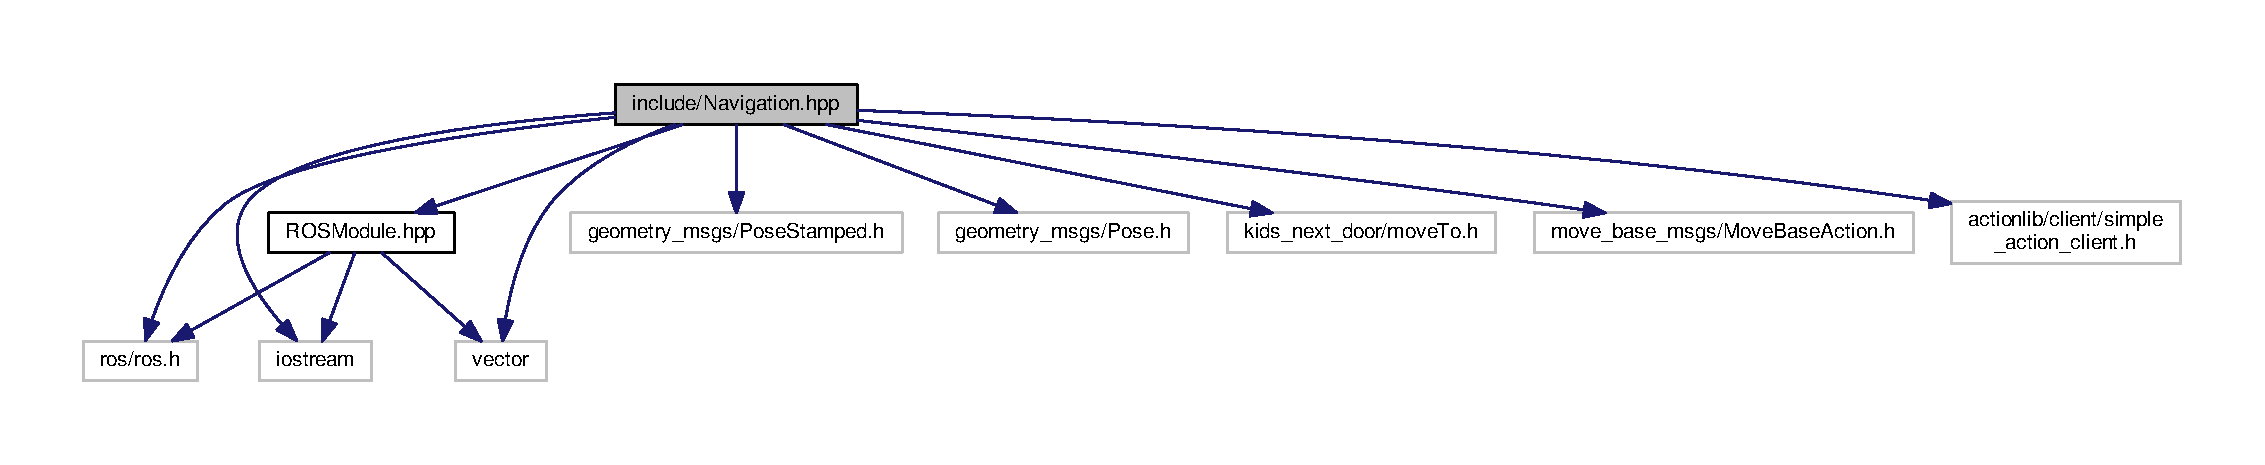
\includegraphics[width=350pt]{Navigation_8hpp__incl}
\end{center}
\end{figure}
This graph shows which files directly or indirectly include this file\+:
\nopagebreak
\begin{figure}[H]
\begin{center}
\leavevmode
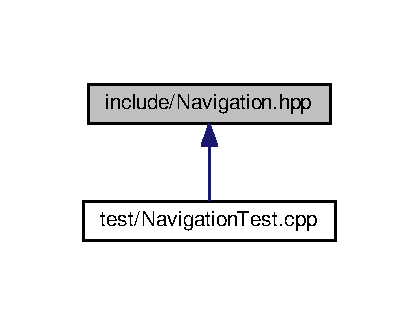
\includegraphics[width=201pt]{Navigation_8hpp__dep__incl}
\end{center}
\end{figure}
\subsection*{Classes}
\begin{DoxyCompactItemize}
\item 
class \hyperlink{classNavigation}{Navigation}
\end{DoxyCompactItemize}


\subsection{Detailed Description}
Header file for \hyperlink{classManipulation}{Manipulation} module. It contains functions and data members required for the manipulation tasks like picking up and placing objects. 

Header file for \hyperlink{classNavigation}{Navigation} Module which contains methods for localization and movement of the robot through the world.

\begin{DoxyAuthor}{Author}
Abhinav Modi 
\end{DoxyAuthor}
\begin{DoxyCopyright}{Copyright}
M\+IT License (c) 2019 Rohan Singh, Abhinav Modi, Ashwin Kuruttukulam 
\end{DoxyCopyright}
\begin{DoxyDate}{Date}
Dec 1, 2019 
\end{DoxyDate}

\hypertarget{ROSModule_8hpp}{}\section{include/\+R\+O\+S\+Module.hpp File Reference}
\label{ROSModule_8hpp}\index{include/\+R\+O\+S\+Module.\+hpp@{include/\+R\+O\+S\+Module.\+hpp}}


Base Header file for R\+OS Modules.  


{\ttfamily \#include $<$iostream$>$}\\*
{\ttfamily \#include $<$vector$>$}\\*
{\ttfamily \#include \char`\"{}ros/ros.\+h\char`\"{}}\\*
Include dependency graph for R\+O\+S\+Module.\+hpp\+:
\nopagebreak
\begin{figure}[H]
\begin{center}
\leavevmode
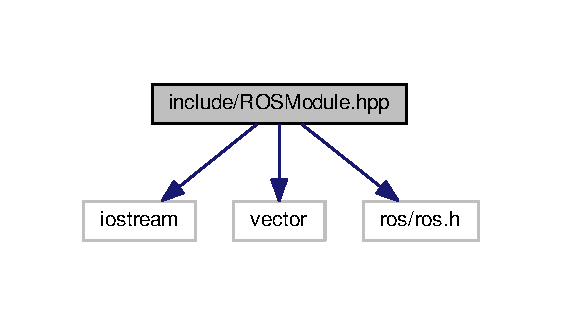
\includegraphics[width=270pt]{ROSModule_8hpp__incl}
\end{center}
\end{figure}
This graph shows which files directly or indirectly include this file\+:
\nopagebreak
\begin{figure}[H]
\begin{center}
\leavevmode
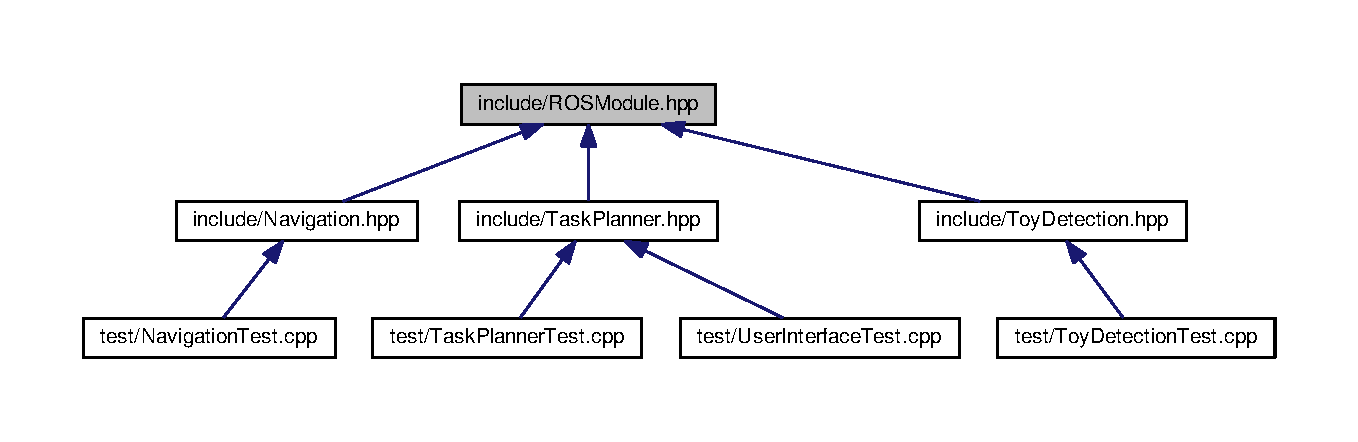
\includegraphics[width=350pt]{ROSModule_8hpp__dep__incl}
\end{center}
\end{figure}
\subsection*{Classes}
\begin{DoxyCompactItemize}
\item 
class \hyperlink{classROSModule}{R\+O\+S\+Module}
\end{DoxyCompactItemize}


\subsection{Detailed Description}
Base Header file for R\+OS Modules. 

\begin{DoxyAuthor}{Author}
Rohan Singh 
\end{DoxyAuthor}
\begin{DoxyCopyright}{Copyright}
M\+IT License (c) 2019 Rohan Singh, Abhinav Modi, Ashwin Kuruttukulam 
\end{DoxyCopyright}
\begin{DoxyDate}{Date}
Dec 6, 2019 
\end{DoxyDate}

\hypertarget{TaskPlanner_8hpp}{}\section{include/\+Task\+Planner.hpp File Reference}
\label{TaskPlanner_8hpp}\index{include/\+Task\+Planner.\+hpp@{include/\+Task\+Planner.\+hpp}}


Header file for Task planner module to make high-\/level decisions for switching between navigation, manipulation and obstacle avoidance tasks.  


{\ttfamily \#include \char`\"{}ros/ros.\+h\char`\"{}}\\*
{\ttfamily \#include \char`\"{}../include/\+R\+O\+S\+Module.\+hpp\char`\"{}}\\*
{\ttfamily \#include \char`\"{}../include/\+User\+Interface.\+hpp\char`\"{}}\\*
{\ttfamily \#include \char`\"{}geometry\+\_\+msgs/\+Pose\+Stamped.\+h\char`\"{}}\\*
{\ttfamily \#include \char`\"{}kids\+\_\+next\+\_\+door/move\+To.\+h\char`\"{}}\\*
{\ttfamily \#include \char`\"{}kids\+\_\+next\+\_\+door/toy\+Found.\+h\char`\"{}}\\*
{\ttfamily \#include $<$iostream$>$}\\*
{\ttfamily \#include $<$vector$>$}\\*
{\ttfamily \#include $<$iterator$>$}\\*
{\ttfamily \#include $<$move\+\_\+base\+\_\+msgs/\+Move\+Base\+Action.\+h$>$}\\*
{\ttfamily \#include $<$actionlib/client/simple\+\_\+action\+\_\+client.\+h$>$}\\*
{\ttfamily \#include $<$boost/shared\+\_\+ptr.\+hpp$>$}\\*
{\ttfamily \#include $<$control\+\_\+msgs/\+Point\+Head\+Action.\+h$>$}\\*
Include dependency graph for Task\+Planner.\+hpp\+:
\nopagebreak
\begin{figure}[H]
\begin{center}
\leavevmode
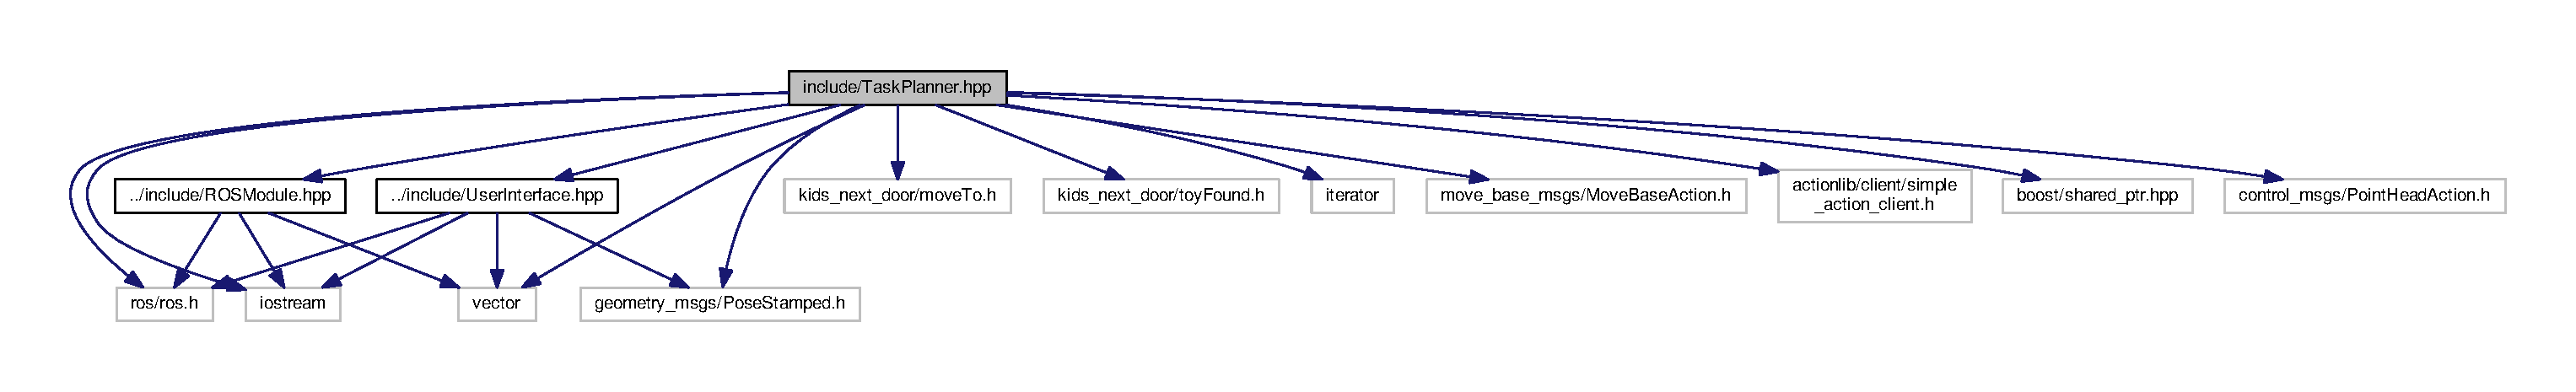
\includegraphics[width=350pt]{TaskPlanner_8hpp__incl}
\end{center}
\end{figure}
This graph shows which files directly or indirectly include this file\+:
\nopagebreak
\begin{figure}[H]
\begin{center}
\leavevmode
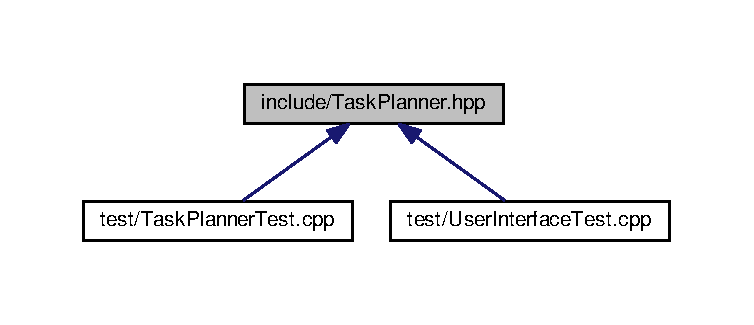
\includegraphics[width=350pt]{TaskPlanner_8hpp__dep__incl}
\end{center}
\end{figure}
\subsection*{Classes}
\begin{DoxyCompactItemize}
\item 
class \hyperlink{classTaskPlanner}{Task\+Planner}
\end{DoxyCompactItemize}


\subsection{Detailed Description}
Header file for Task planner module to make high-\/level decisions for switching between navigation, manipulation and obstacle avoidance tasks. 

\begin{DoxyAuthor}{Author}
Abhinav Modi 
\end{DoxyAuthor}
\begin{DoxyCopyright}{Copyright}
M\+IT License (c) 2019 Rohan Singh, Abhinav Modi, Ashwin Kuruttukulam 
\end{DoxyCopyright}
\begin{DoxyDate}{Date}
Dec 1, 2019 
\end{DoxyDate}

\hypertarget{ToyDetection_8hpp}{}\section{include/\+Toy\+Detection.hpp File Reference}
\label{ToyDetection_8hpp}\index{include/\+Toy\+Detection.\+hpp@{include/\+Toy\+Detection.\+hpp}}


Header file for \hyperlink{classToyDetection}{Toy\+Detection} module to detect and locate toys in the robot\textquotesingle{}s base frame using Ar\+Uco markers present on the toys.  


{\ttfamily \#include $<$iostream$>$}\\*
{\ttfamily \#include $<$vector$>$}\\*
{\ttfamily \#include \char`\"{}../include/\+R\+O\+S\+Module.\+hpp\char`\"{}}\\*
{\ttfamily \#include $<$tf/transform\+\_\+listener.\+h$>$}\\*
{\ttfamily \#include \char`\"{}ros/ros.\+h\char`\"{}}\\*
{\ttfamily \#include \char`\"{}geometry\+\_\+msgs/\+Pose\+Stamped.\+h\char`\"{}}\\*
{\ttfamily \#include \char`\"{}kids\+\_\+next\+\_\+door/toy\+Found.\+h\char`\"{}}\\*
Include dependency graph for Toy\+Detection.\+hpp\+:
\nopagebreak
\begin{figure}[H]
\begin{center}
\leavevmode
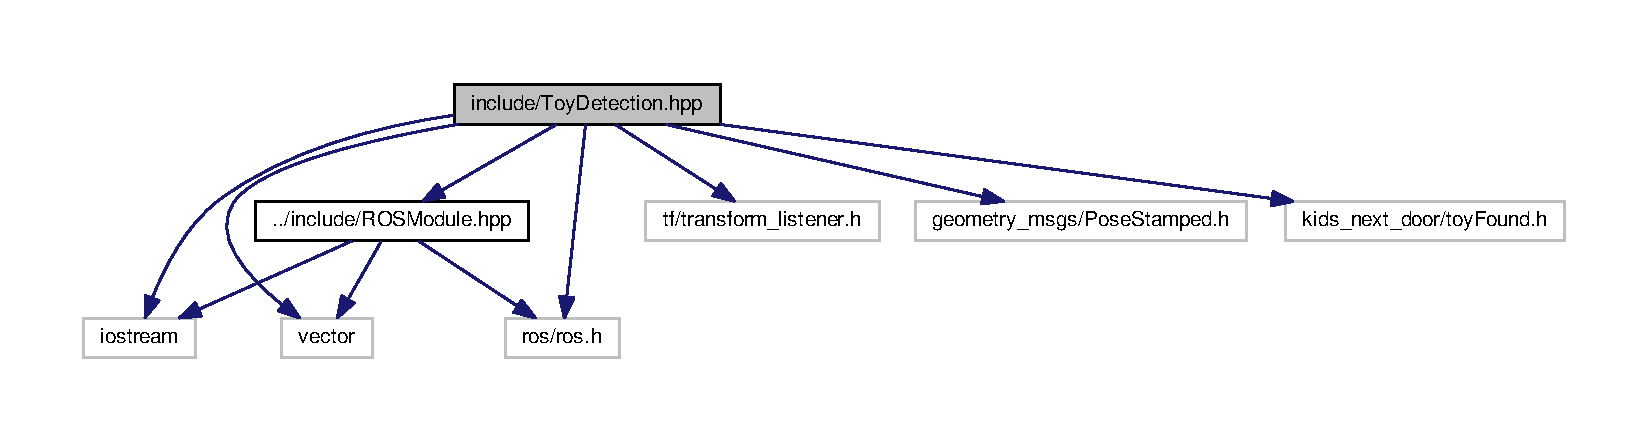
\includegraphics[width=350pt]{ToyDetection_8hpp__incl}
\end{center}
\end{figure}
This graph shows which files directly or indirectly include this file\+:
\nopagebreak
\begin{figure}[H]
\begin{center}
\leavevmode
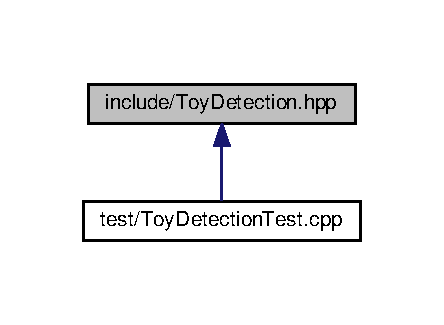
\includegraphics[width=213pt]{ToyDetection_8hpp__dep__incl}
\end{center}
\end{figure}
\subsection*{Classes}
\begin{DoxyCompactItemize}
\item 
class \hyperlink{classToyDetection}{Toy\+Detection}
\end{DoxyCompactItemize}


\subsection{Detailed Description}
Header file for \hyperlink{classToyDetection}{Toy\+Detection} module to detect and locate toys in the robot\textquotesingle{}s base frame using Ar\+Uco markers present on the toys. 

\begin{DoxyAuthor}{Author}
Abhinav Modi 
\end{DoxyAuthor}
\begin{DoxyCopyright}{Copyright}
M\+IT License (c) 2019 Rohan Singh, Abhinav Modi, Ashwin Kuruttukulam 
\end{DoxyCopyright}
\begin{DoxyDate}{Date}
Dec 1, 2019 
\end{DoxyDate}

\hypertarget{UserInterface_8hpp}{}\section{include/\+User\+Interface.hpp File Reference}
\label{UserInterface_8hpp}\index{include/\+User\+Interface.\+hpp@{include/\+User\+Interface.\+hpp}}


Header file for \hyperlink{classUserInterface}{User\+Interface} Class.  


{\ttfamily \#include $<$iostream$>$}\\*
{\ttfamily \#include $<$vector$>$}\\*
{\ttfamily \#include \char`\"{}ros/ros.\+h\char`\"{}}\\*
{\ttfamily \#include \char`\"{}geometry\+\_\+msgs/\+Pose\+Stamped.\+h\char`\"{}}\\*
Include dependency graph for User\+Interface.\+hpp\+:
\nopagebreak
\begin{figure}[H]
\begin{center}
\leavevmode
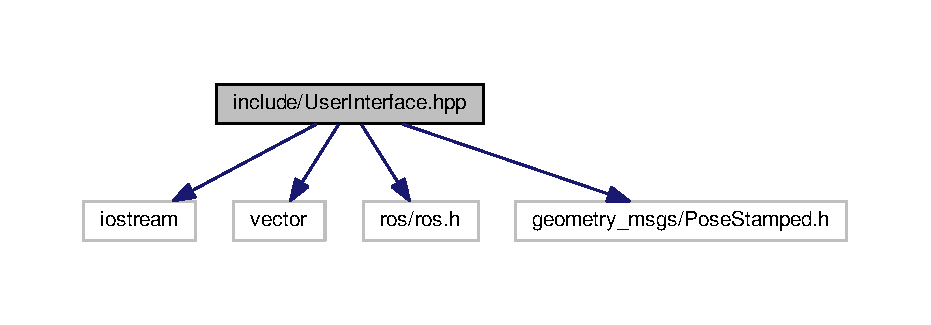
\includegraphics[width=350pt]{UserInterface_8hpp__incl}
\end{center}
\end{figure}
This graph shows which files directly or indirectly include this file\+:
\nopagebreak
\begin{figure}[H]
\begin{center}
\leavevmode
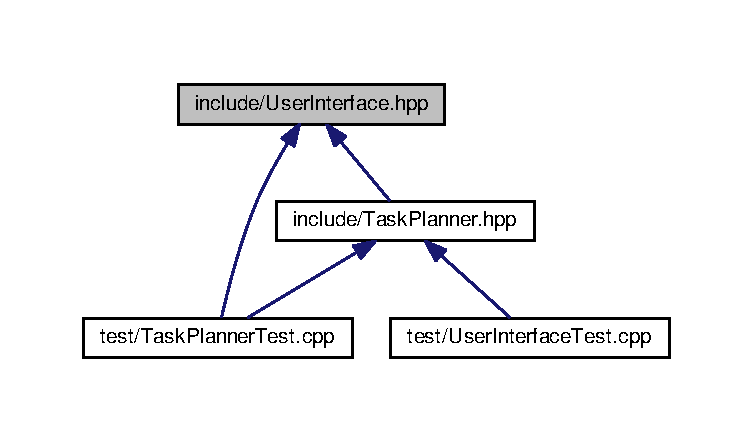
\includegraphics[width=350pt]{UserInterface_8hpp__dep__incl}
\end{center}
\end{figure}
\subsection*{Classes}
\begin{DoxyCompactItemize}
\item 
class \hyperlink{classUserInterface}{User\+Interface}
\end{DoxyCompactItemize}


\subsection{Detailed Description}
Header file for \hyperlink{classUserInterface}{User\+Interface} Class. 

\begin{DoxyAuthor}{Author}
Rohan Singh 
\end{DoxyAuthor}
\begin{DoxyCopyright}{Copyright}
M\+IT License (c) 2019 Rohan Singh, Abhinav Modi, Ashwin Kuruttukulam 
\end{DoxyCopyright}
\begin{DoxyDate}{Date}
Dec 9, 2019 
\end{DoxyDate}

\hypertarget{ManipulationTest_8cpp}{}\section{test/\+Manipulation\+Test.cpp File Reference}
\label{ManipulationTest_8cpp}\index{test/\+Manipulation\+Test.\+cpp@{test/\+Manipulation\+Test.\+cpp}}


Unit tests for class \hyperlink{classManipulation}{Manipulation}.  


{\ttfamily \#include $<$gtest/gtest.\+h$>$}\\*
{\ttfamily \#include \char`\"{}Manipulation.\+hpp\char`\"{}}\\*
Include dependency graph for Manipulation\+Test.\+cpp\+:
\nopagebreak
\begin{figure}[H]
\begin{center}
\leavevmode
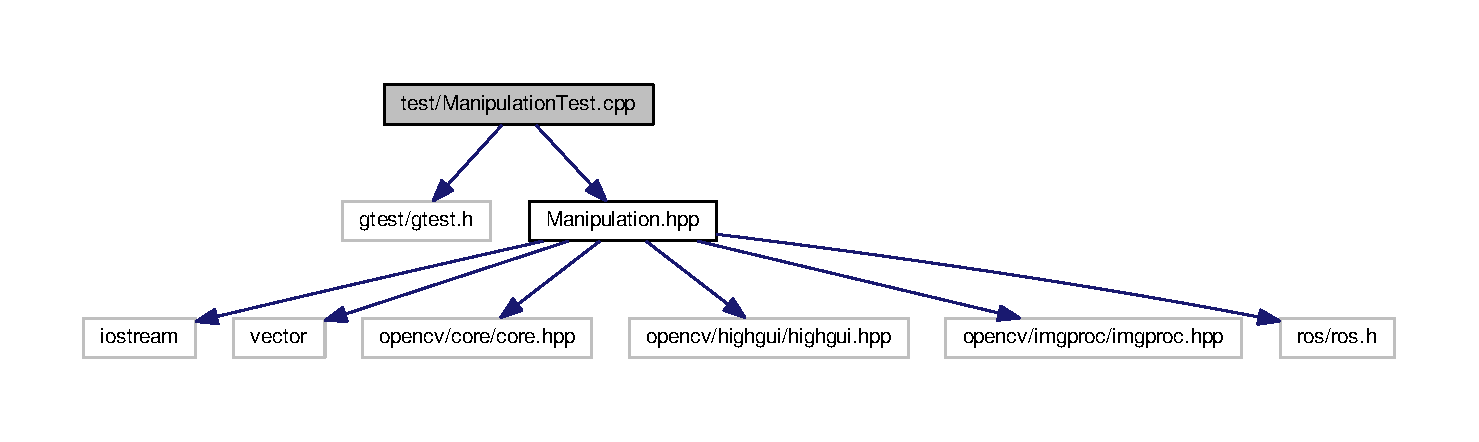
\includegraphics[width=350pt]{ManipulationTest_8cpp__incl}
\end{center}
\end{figure}
\subsection*{Functions}
\begin{DoxyCompactItemize}
\item 
\hyperlink{ManipulationTest_8cpp_a07e3b11123581dc3cdad615e4d9a501c}{T\+E\+ST} (Manipulation\+Class\+Test, Test\+Get\+Toy\+Position)
\begin{DoxyCompactList}\small\item\em Test to check get\+Toy\+Position functionality. \end{DoxyCompactList}\item 
\hyperlink{ManipulationTest_8cpp_a82f37211807a647f9f8e3355f0add47f}{T\+E\+ST} (Manipulation\+Class\+Test, Test\+Pickup)
\begin{DoxyCompactList}\small\item\em Test to check pickup functionality. \end{DoxyCompactList}\item 
\hyperlink{ManipulationTest_8cpp_ab7576f1c4d87e29cfbd385e945221c83}{T\+E\+ST} (Manipulation\+Class\+Test, Test\+Drop)
\begin{DoxyCompactList}\small\item\em Test to check drop functionality. \end{DoxyCompactList}\end{DoxyCompactItemize}


\subsection{Detailed Description}
Unit tests for class \hyperlink{classManipulation}{Manipulation}. 

\begin{DoxyAuthor}{Author}
Rohan Singh 
\end{DoxyAuthor}
\begin{DoxyCopyright}{Copyright}
M\+IT License (c) 2019 Rohan Singh, Abhinav Modi, Ashwin Kuruttukulam 
\end{DoxyCopyright}
\begin{DoxyDate}{Date}
Dec 1, 2019 
\end{DoxyDate}


\subsection{Function Documentation}
\index{Manipulation\+Test.\+cpp@{Manipulation\+Test.\+cpp}!T\+E\+ST@{T\+E\+ST}}
\index{T\+E\+ST@{T\+E\+ST}!Manipulation\+Test.\+cpp@{Manipulation\+Test.\+cpp}}
\subsubsection[{\texorpdfstring{T\+E\+S\+T(\+Manipulation\+Class\+Test, Test\+Get\+Toy\+Position)}{TEST(ManipulationClassTest, TestGetToyPosition)}}]{\setlength{\rightskip}{0pt plus 5cm}T\+E\+ST (
\begin{DoxyParamCaption}
\item[{Manipulation\+Class\+Test}]{, }
\item[{Test\+Get\+Toy\+Position}]{}
\end{DoxyParamCaption}
)}\hypertarget{ManipulationTest_8cpp_a07e3b11123581dc3cdad615e4d9a501c}{}\label{ManipulationTest_8cpp_a07e3b11123581dc3cdad615e4d9a501c}


Test to check get\+Toy\+Position functionality. 


\begin{DoxyParams}{Parameters}
{\em none} & \\
\hline
\end{DoxyParams}
\begin{DoxyReturn}{Returns}
none 
\end{DoxyReturn}
\index{Manipulation\+Test.\+cpp@{Manipulation\+Test.\+cpp}!T\+E\+ST@{T\+E\+ST}}
\index{T\+E\+ST@{T\+E\+ST}!Manipulation\+Test.\+cpp@{Manipulation\+Test.\+cpp}}
\subsubsection[{\texorpdfstring{T\+E\+S\+T(\+Manipulation\+Class\+Test, Test\+Pickup)}{TEST(ManipulationClassTest, TestPickup)}}]{\setlength{\rightskip}{0pt plus 5cm}T\+E\+ST (
\begin{DoxyParamCaption}
\item[{Manipulation\+Class\+Test}]{, }
\item[{Test\+Pickup}]{}
\end{DoxyParamCaption}
)}\hypertarget{ManipulationTest_8cpp_a82f37211807a647f9f8e3355f0add47f}{}\label{ManipulationTest_8cpp_a82f37211807a647f9f8e3355f0add47f}


Test to check pickup functionality. 


\begin{DoxyParams}{Parameters}
{\em none} & \\
\hline
\end{DoxyParams}
\begin{DoxyReturn}{Returns}
none 
\end{DoxyReturn}
\index{Manipulation\+Test.\+cpp@{Manipulation\+Test.\+cpp}!T\+E\+ST@{T\+E\+ST}}
\index{T\+E\+ST@{T\+E\+ST}!Manipulation\+Test.\+cpp@{Manipulation\+Test.\+cpp}}
\subsubsection[{\texorpdfstring{T\+E\+S\+T(\+Manipulation\+Class\+Test, Test\+Drop)}{TEST(ManipulationClassTest, TestDrop)}}]{\setlength{\rightskip}{0pt plus 5cm}T\+E\+ST (
\begin{DoxyParamCaption}
\item[{Manipulation\+Class\+Test}]{, }
\item[{Test\+Drop}]{}
\end{DoxyParamCaption}
)}\hypertarget{ManipulationTest_8cpp_ab7576f1c4d87e29cfbd385e945221c83}{}\label{ManipulationTest_8cpp_ab7576f1c4d87e29cfbd385e945221c83}


Test to check drop functionality. 


\begin{DoxyParams}{Parameters}
{\em none} & \\
\hline
\end{DoxyParams}
\begin{DoxyReturn}{Returns}
none 
\end{DoxyReturn}

\hypertarget{NavigationTest_8cpp}{}\section{test/\+Navigation\+Test.cpp File Reference}
\label{NavigationTest_8cpp}\index{test/\+Navigation\+Test.\+cpp@{test/\+Navigation\+Test.\+cpp}}


Unit tests for class \hyperlink{classNavigation}{Navigation}.  


{\ttfamily \#include $<$gtest/gtest.\+h$>$}\\*
{\ttfamily \#include \char`\"{}../include/\+Navigation.\+hpp\char`\"{}}\\*
Include dependency graph for Navigation\+Test.\+cpp\+:
\nopagebreak
\begin{figure}[H]
\begin{center}
\leavevmode
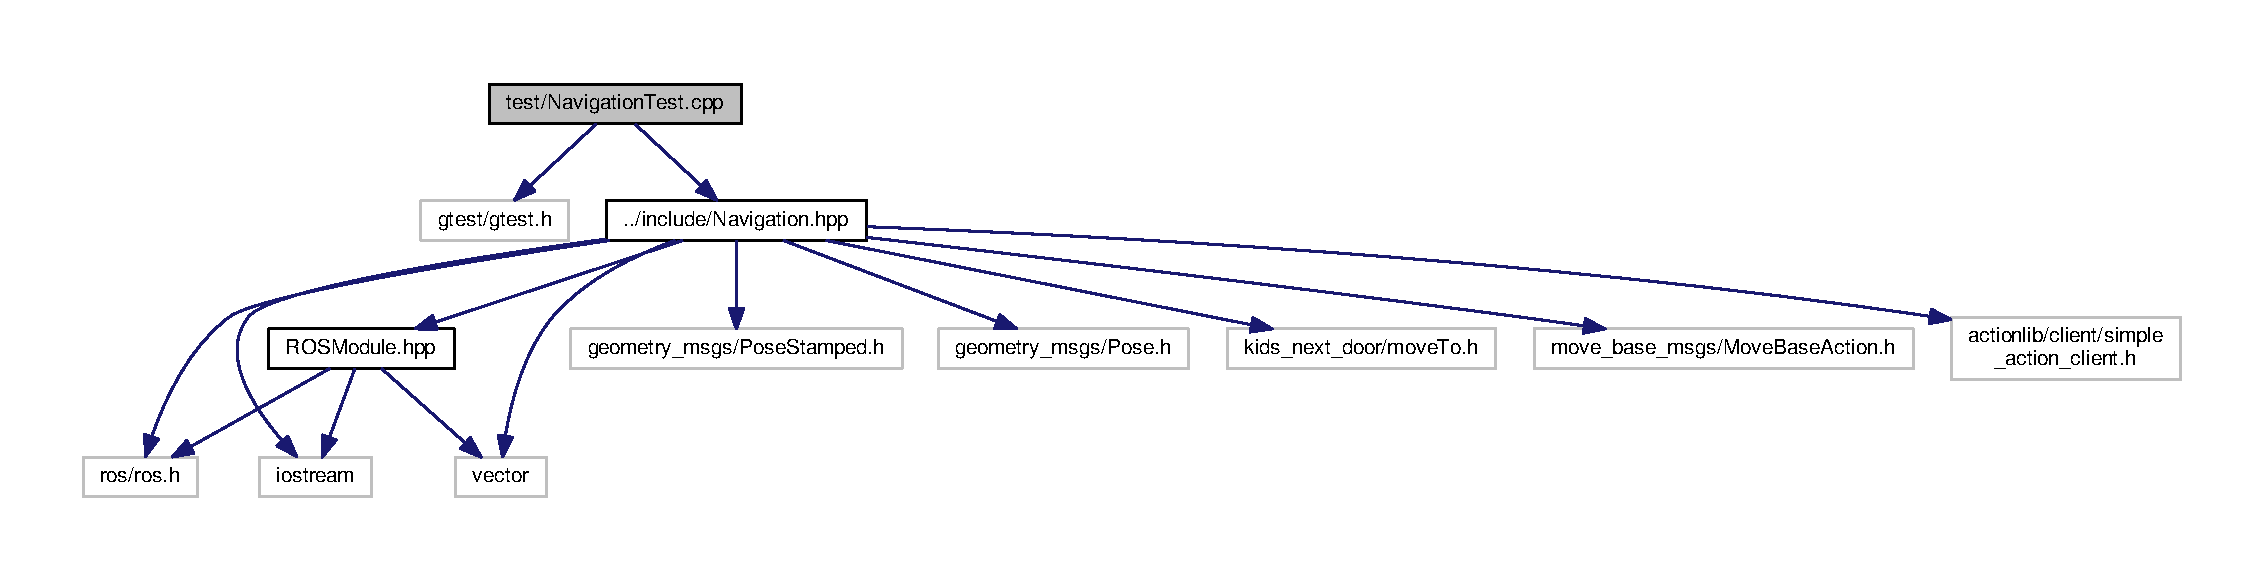
\includegraphics[width=350pt]{NavigationTest_8cpp__incl}
\end{center}
\end{figure}
\subsection*{Functions}
\begin{DoxyCompactItemize}
\item 
\hyperlink{NavigationTest_8cpp_aebaa5372082acccb9dbfb23a13fc513e}{T\+E\+ST} (Navigation\+Class\+Test, Test\+Move\+To\+Service)\hypertarget{NavigationTest_8cpp_aebaa5372082acccb9dbfb23a13fc513e}{}\label{NavigationTest_8cpp_aebaa5372082acccb9dbfb23a13fc513e}

\begin{DoxyCompactList}\small\item\em Test to check move\+To service. \end{DoxyCompactList}\item 
\hyperlink{NavigationTest_8cpp_ab929d5fae5978a3565b2c2cdf7112968}{T\+E\+ST} (Navigation\+Class\+Test, Test\+Set\+Goal\+Method)\hypertarget{NavigationTest_8cpp_ab929d5fae5978a3565b2c2cdf7112968}{}\label{NavigationTest_8cpp_ab929d5fae5978a3565b2c2cdf7112968}

\begin{DoxyCompactList}\small\item\em Test to check set\+Goal method to set goal to a received pose during the service call. \end{DoxyCompactList}\end{DoxyCompactItemize}


\subsection{Detailed Description}
Unit tests for class \hyperlink{classNavigation}{Navigation}. 

\begin{DoxyAuthor}{Author}
Rohan Singh 
\end{DoxyAuthor}
\begin{DoxyCopyright}{Copyright}
M\+IT License (c) 2019 Rohan Singh, Abhinav Modi, Ashwin Kuruttukulam 
\end{DoxyCopyright}
\begin{DoxyDate}{Date}
Dec 1, 2019 
\end{DoxyDate}

\hypertarget{TaskPlannerTest_8cpp}{}\section{test/\+Task\+Planner\+Test.cpp File Reference}
\label{TaskPlannerTest_8cpp}\index{test/\+Task\+Planner\+Test.\+cpp@{test/\+Task\+Planner\+Test.\+cpp}}


Unit tests for class \hyperlink{classTaskPlanner}{Task\+Planner}.  


{\ttfamily \#include $<$gtest/gtest.\+h$>$}\\*
{\ttfamily \#include $<$sstream$>$}\\*
{\ttfamily \#include \char`\"{}../include/\+Task\+Planner.\+hpp\char`\"{}}\\*
{\ttfamily \#include \char`\"{}../include/\+User\+Interface.\+hpp\char`\"{}}\\*
{\ttfamily \#include \char`\"{}ros/ros.\+h\char`\"{}}\\*
{\ttfamily \#include \char`\"{}ros/service\+\_\+client.\+h\char`\"{}}\\*
Include dependency graph for Task\+Planner\+Test.\+cpp\+:
\nopagebreak
\begin{figure}[H]
\begin{center}
\leavevmode
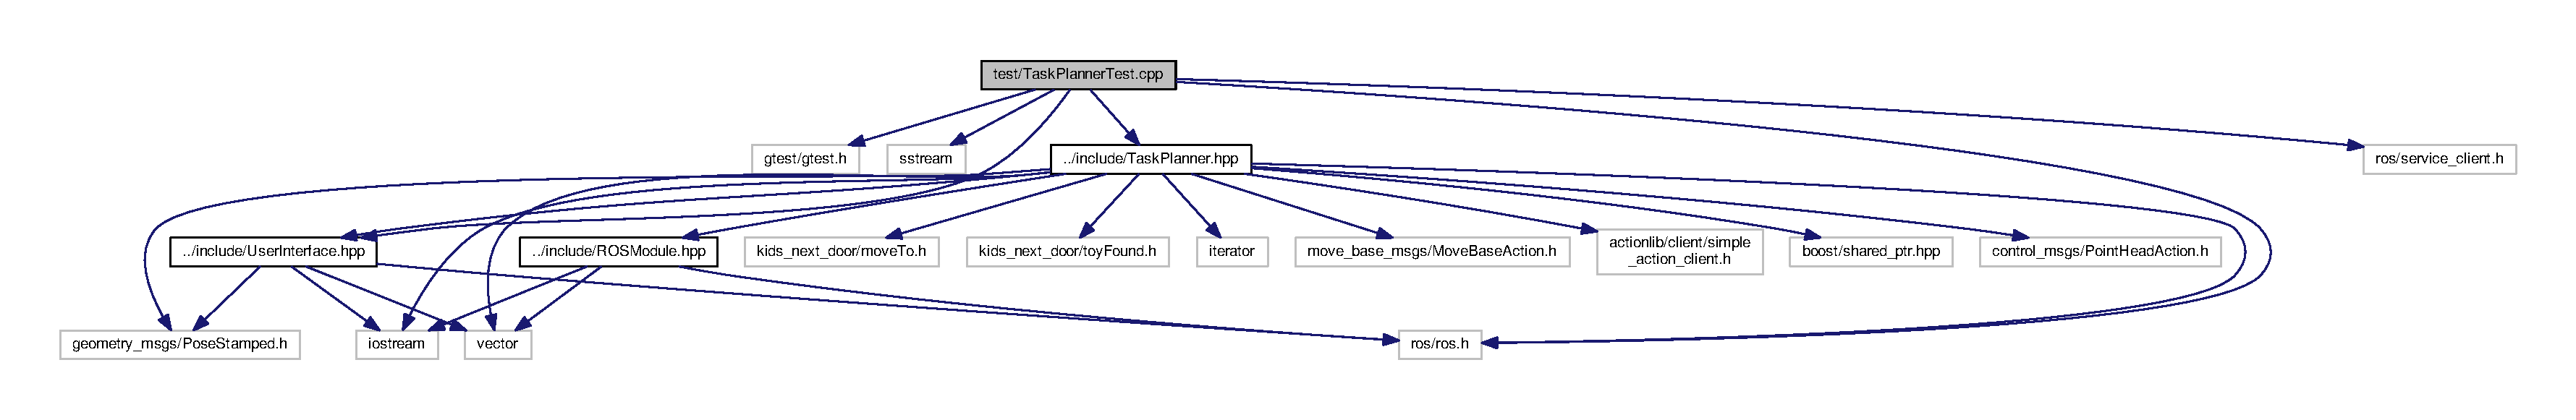
\includegraphics[width=350pt]{TaskPlannerTest_8cpp__incl}
\end{center}
\end{figure}
\subsection*{Functions}
\begin{DoxyCompactItemize}
\item 
\hyperlink{TaskPlannerTest_8cpp_a1a33f19c6a92304d289f2676ceb9391d}{T\+E\+ST} (Task\+Planner\+Class\+Test, Test\+Main\+Node)
\begin{DoxyCompactList}\small\item\em Test to main Node functionality. \end{DoxyCompactList}\item 
\hyperlink{TaskPlannerTest_8cpp_a41b09c92ff801907d911ceb36fb1d284}{T\+E\+ST} (Task\+Planner\+Class\+Test, Test\+Move\+To\+Pose)
\begin{DoxyCompactList}\small\item\em Test to check move\+To functionality. \end{DoxyCompactList}\item 
\hyperlink{TaskPlannerTest_8cpp_a56de67c46fb4fd9ff7b31efb96d04704}{T\+E\+ST} (Task\+Planner\+Class\+Test, Test\+Look\+For\+Toy)
\begin{DoxyCompactList}\small\item\em Test to check look\+For\+Toy functionality. \end{DoxyCompactList}\end{DoxyCompactItemize}


\subsection{Detailed Description}
Unit tests for class \hyperlink{classTaskPlanner}{Task\+Planner}. 

\begin{DoxyAuthor}{Author}
Rohan Singh 
\end{DoxyAuthor}
\begin{DoxyCopyright}{Copyright}
M\+IT License (c) 2019 Rohan Singh, Abhinav Modi, Ashwin Kuruttukulam 
\end{DoxyCopyright}
\begin{DoxyDate}{Date}
Dec 1, 2019 
\end{DoxyDate}


\subsection{Function Documentation}
\index{Task\+Planner\+Test.\+cpp@{Task\+Planner\+Test.\+cpp}!T\+E\+ST@{T\+E\+ST}}
\index{T\+E\+ST@{T\+E\+ST}!Task\+Planner\+Test.\+cpp@{Task\+Planner\+Test.\+cpp}}
\subsubsection[{\texorpdfstring{T\+E\+S\+T(\+Task\+Planner\+Class\+Test, Test\+Main\+Node)}{TEST(TaskPlannerClassTest, TestMainNode)}}]{\setlength{\rightskip}{0pt plus 5cm}T\+E\+ST (
\begin{DoxyParamCaption}
\item[{Task\+Planner\+Class\+Test}]{, }
\item[{Test\+Main\+Node}]{}
\end{DoxyParamCaption}
)}\hypertarget{TaskPlannerTest_8cpp_a1a33f19c6a92304d289f2676ceb9391d}{}\label{TaskPlannerTest_8cpp_a1a33f19c6a92304d289f2676ceb9391d}


Test to main Node functionality. 


\begin{DoxyParams}{Parameters}
{\em none} & \\
\hline
\end{DoxyParams}
\begin{DoxyReturn}{Returns}
none 
\end{DoxyReturn}
\index{Task\+Planner\+Test.\+cpp@{Task\+Planner\+Test.\+cpp}!T\+E\+ST@{T\+E\+ST}}
\index{T\+E\+ST@{T\+E\+ST}!Task\+Planner\+Test.\+cpp@{Task\+Planner\+Test.\+cpp}}
\subsubsection[{\texorpdfstring{T\+E\+S\+T(\+Task\+Planner\+Class\+Test, Test\+Move\+To\+Pose)}{TEST(TaskPlannerClassTest, TestMoveToPose)}}]{\setlength{\rightskip}{0pt plus 5cm}T\+E\+ST (
\begin{DoxyParamCaption}
\item[{Task\+Planner\+Class\+Test}]{, }
\item[{Test\+Move\+To\+Pose}]{}
\end{DoxyParamCaption}
)}\hypertarget{TaskPlannerTest_8cpp_a41b09c92ff801907d911ceb36fb1d284}{}\label{TaskPlannerTest_8cpp_a41b09c92ff801907d911ceb36fb1d284}


Test to check move\+To functionality. 


\begin{DoxyParams}{Parameters}
{\em none} & \\
\hline
\end{DoxyParams}
\begin{DoxyReturn}{Returns}
none 
\end{DoxyReturn}
\index{Task\+Planner\+Test.\+cpp@{Task\+Planner\+Test.\+cpp}!T\+E\+ST@{T\+E\+ST}}
\index{T\+E\+ST@{T\+E\+ST}!Task\+Planner\+Test.\+cpp@{Task\+Planner\+Test.\+cpp}}
\subsubsection[{\texorpdfstring{T\+E\+S\+T(\+Task\+Planner\+Class\+Test, Test\+Look\+For\+Toy)}{TEST(TaskPlannerClassTest, TestLookForToy)}}]{\setlength{\rightskip}{0pt plus 5cm}T\+E\+ST (
\begin{DoxyParamCaption}
\item[{Task\+Planner\+Class\+Test}]{, }
\item[{Test\+Look\+For\+Toy}]{}
\end{DoxyParamCaption}
)}\hypertarget{TaskPlannerTest_8cpp_a56de67c46fb4fd9ff7b31efb96d04704}{}\label{TaskPlannerTest_8cpp_a56de67c46fb4fd9ff7b31efb96d04704}


Test to check look\+For\+Toy functionality. 


\begin{DoxyParams}{Parameters}
{\em none} & \\
\hline
\end{DoxyParams}
\begin{DoxyReturn}{Returns}
none 
\end{DoxyReturn}

\hypertarget{ToyDetectionTest_8cpp}{}\section{test/\+Toy\+Detection\+Test.cpp File Reference}
\label{ToyDetectionTest_8cpp}\index{test/\+Toy\+Detection\+Test.\+cpp@{test/\+Toy\+Detection\+Test.\+cpp}}


Unit tests for class \hyperlink{classToyDetection}{Toy\+Detection}.  


{\ttfamily \#include $<$gtest/gtest.\+h$>$}\\*
{\ttfamily \#include \char`\"{}Toy\+Detection.\+hpp\char`\"{}}\\*
Include dependency graph for Toy\+Detection\+Test.\+cpp\+:
\nopagebreak
\begin{figure}[H]
\begin{center}
\leavevmode
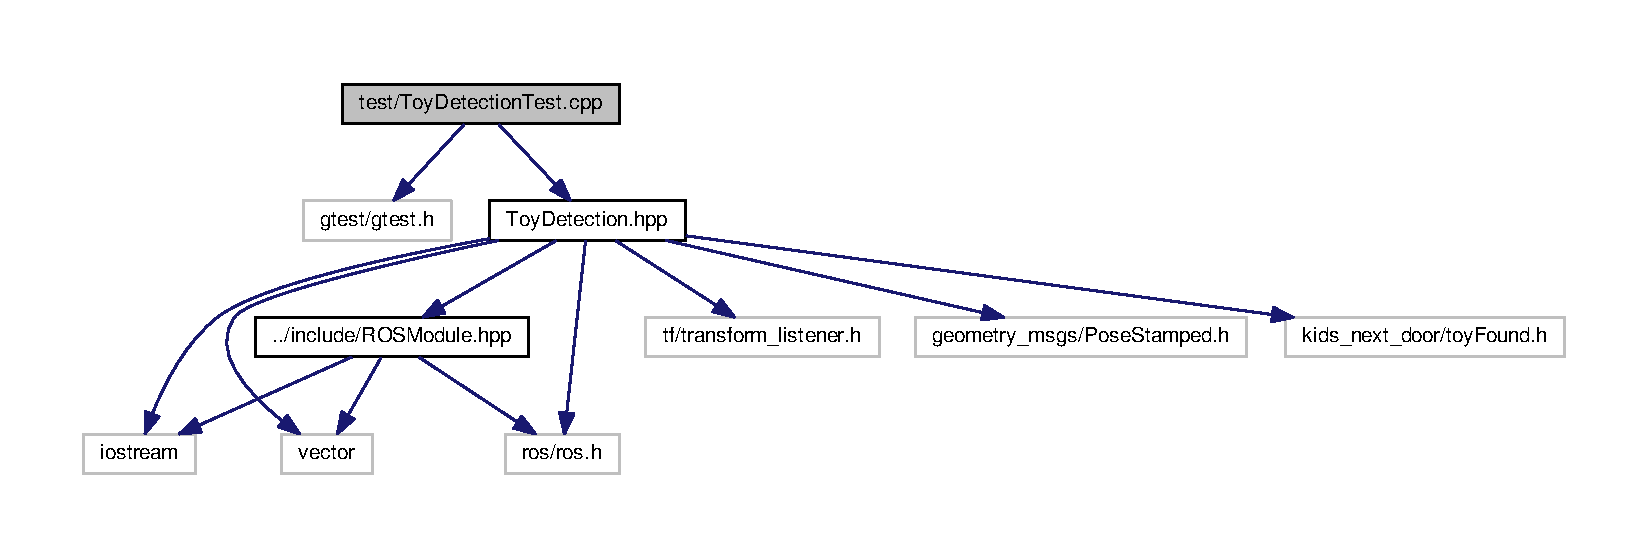
\includegraphics[width=350pt]{ToyDetectionTest_8cpp__incl}
\end{center}
\end{figure}
\subsection*{Functions}
\begin{DoxyCompactItemize}
\item 
\hyperlink{ToyDetectionTest_8cpp_ad7aae0f06d89f19067030a16fe8b04d5}{T\+E\+ST} (Toy\+Detection\+Class\+Test, Find\+Toy\+Service\+Test)\hypertarget{ToyDetectionTest_8cpp_ad7aae0f06d89f19067030a16fe8b04d5}{}\label{ToyDetectionTest_8cpp_ad7aae0f06d89f19067030a16fe8b04d5}

\begin{DoxyCompactList}\small\item\em Test to check toy\+Found Service. \end{DoxyCompactList}\item 
\hyperlink{ToyDetectionTest_8cpp_a39bfb5d531cd6438118868693b05b147}{T\+E\+ST} (Toy\+Detection\+Class\+Test, detect\+Aruco\+Test)
\begin{DoxyCompactList}\small\item\em Test to check toy\+Position\+Pub functionality. \end{DoxyCompactList}\item 
\hyperlink{ToyDetectionTest_8cpp_a9f3078ed4bc5753ffc5c11973d47b533}{T\+E\+ST} (Toy\+Detection\+Class\+Test, Successful\+Initialization)\hypertarget{ToyDetectionTest_8cpp_a9f3078ed4bc5753ffc5c11973d47b533}{}\label{ToyDetectionTest_8cpp_a9f3078ed4bc5753ffc5c11973d47b533}

\begin{DoxyCompactList}\small\item\em Test to check successful initialization of the module. \end{DoxyCompactList}\end{DoxyCompactItemize}


\subsection{Detailed Description}
Unit tests for class \hyperlink{classToyDetection}{Toy\+Detection}. 

\begin{DoxyAuthor}{Author}
Rohan Singh 
\end{DoxyAuthor}
\begin{DoxyCopyright}{Copyright}
M\+IT License (c) 2019 Rohan Singh, Abhinav Modi, Ashwin Kuruttukulam 
\end{DoxyCopyright}
\begin{DoxyDate}{Date}
Dec 1, 2019 
\end{DoxyDate}


\subsection{Function Documentation}
\index{Toy\+Detection\+Test.\+cpp@{Toy\+Detection\+Test.\+cpp}!T\+E\+ST@{T\+E\+ST}}
\index{T\+E\+ST@{T\+E\+ST}!Toy\+Detection\+Test.\+cpp@{Toy\+Detection\+Test.\+cpp}}
\subsubsection[{\texorpdfstring{T\+E\+S\+T(\+Toy\+Detection\+Class\+Test, detect\+Aruco\+Test)}{TEST(ToyDetectionClassTest, detectArucoTest)}}]{\setlength{\rightskip}{0pt plus 5cm}T\+E\+ST (
\begin{DoxyParamCaption}
\item[{Toy\+Detection\+Class\+Test}]{, }
\item[{detect\+Aruco\+Test}]{}
\end{DoxyParamCaption}
)}\hypertarget{ToyDetectionTest_8cpp_a39bfb5d531cd6438118868693b05b147}{}\label{ToyDetectionTest_8cpp_a39bfb5d531cd6438118868693b05b147}


Test to check toy\+Position\+Pub functionality. 


\begin{DoxyParams}{Parameters}
{\em none} & \\
\hline
\end{DoxyParams}
\begin{DoxyReturn}{Returns}
none 
\end{DoxyReturn}

\hypertarget{UserInterfaceTest_8cpp}{}\section{test/\+User\+Interface\+Test.cpp File Reference}
\label{UserInterfaceTest_8cpp}\index{test/\+User\+Interface\+Test.\+cpp@{test/\+User\+Interface\+Test.\+cpp}}


Unit tests for class \hyperlink{classUserInterface}{User\+Interface}.  


{\ttfamily \#include $<$gtest/gtest.\+h$>$}\\*
{\ttfamily \#include $<$sstream$>$}\\*
{\ttfamily \#include \char`\"{}../include/\+Task\+Planner.\+hpp\char`\"{}}\\*
{\ttfamily \#include \char`\"{}ros/ros.\+h\char`\"{}}\\*
{\ttfamily \#include \char`\"{}geometry\+\_\+msgs/\+Pose\+Stamped.\+h\char`\"{}}\\*
Include dependency graph for User\+Interface\+Test.\+cpp\+:
\nopagebreak
\begin{figure}[H]
\begin{center}
\leavevmode
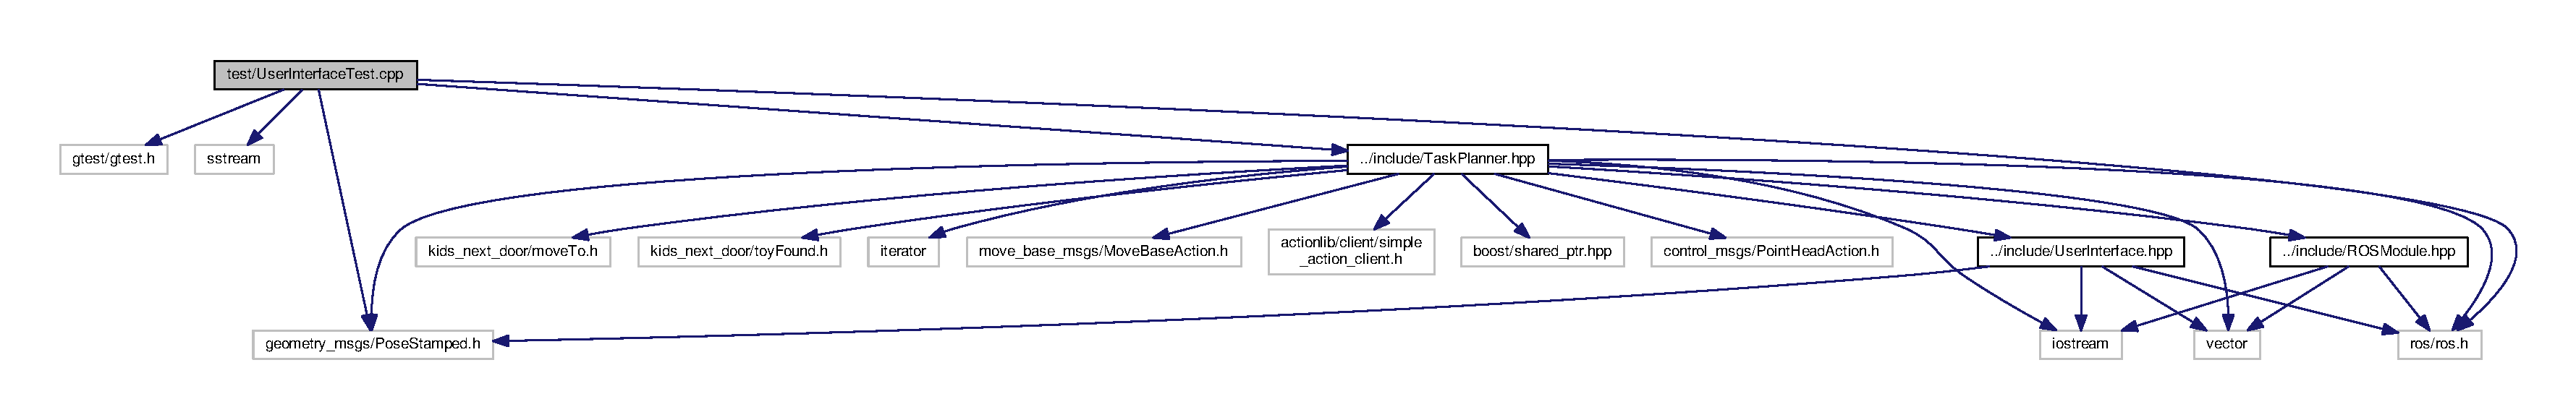
\includegraphics[width=350pt]{UserInterfaceTest_8cpp__incl}
\end{center}
\end{figure}
\subsection*{Functions}
\begin{DoxyCompactItemize}
\item 
\hyperlink{UserInterfaceTest_8cpp_a44326d0582f7263e371c862d12f0179b}{T\+E\+ST} (User\+Interface\+Class\+Test, Test\+Get\+I\+Ds)
\begin{DoxyCompactList}\small\item\em Test to check get\+I\+Ds functionality. \end{DoxyCompactList}\item 
\hyperlink{UserInterfaceTest_8cpp_a047196dee91cd0f211b04cdcb357380f}{T\+E\+ST} (User\+Interface\+Class\+Test, Test\+Look\+For\+Toy)
\begin{DoxyCompactList}\small\item\em Test to check get\+Storage\+Location functionality. \end{DoxyCompactList}\end{DoxyCompactItemize}


\subsection{Detailed Description}
Unit tests for class \hyperlink{classUserInterface}{User\+Interface}. 

\begin{DoxyAuthor}{Author}
Rohan Singh 
\end{DoxyAuthor}
\begin{DoxyCopyright}{Copyright}
M\+IT License (c) 2019 Rohan Singh, Abhinav Modi, Ashwin Kuruttukulam 
\end{DoxyCopyright}
\begin{DoxyDate}{Date}
Dec 1, 2019 
\end{DoxyDate}


\subsection{Function Documentation}
\index{User\+Interface\+Test.\+cpp@{User\+Interface\+Test.\+cpp}!T\+E\+ST@{T\+E\+ST}}
\index{T\+E\+ST@{T\+E\+ST}!User\+Interface\+Test.\+cpp@{User\+Interface\+Test.\+cpp}}
\subsubsection[{\texorpdfstring{T\+E\+S\+T(\+User\+Interface\+Class\+Test, Test\+Get\+I\+Ds)}{TEST(UserInterfaceClassTest, TestGetIDs)}}]{\setlength{\rightskip}{0pt plus 5cm}T\+E\+ST (
\begin{DoxyParamCaption}
\item[{User\+Interface\+Class\+Test}]{, }
\item[{Test\+Get\+I\+Ds}]{}
\end{DoxyParamCaption}
)}\hypertarget{UserInterfaceTest_8cpp_a44326d0582f7263e371c862d12f0179b}{}\label{UserInterfaceTest_8cpp_a44326d0582f7263e371c862d12f0179b}


Test to check get\+I\+Ds functionality. 


\begin{DoxyParams}{Parameters}
{\em None} & \\
\hline
\end{DoxyParams}
\begin{DoxyReturn}{Returns}
none 
\end{DoxyReturn}
\index{User\+Interface\+Test.\+cpp@{User\+Interface\+Test.\+cpp}!T\+E\+ST@{T\+E\+ST}}
\index{T\+E\+ST@{T\+E\+ST}!User\+Interface\+Test.\+cpp@{User\+Interface\+Test.\+cpp}}
\subsubsection[{\texorpdfstring{T\+E\+S\+T(\+User\+Interface\+Class\+Test, Test\+Look\+For\+Toy)}{TEST(UserInterfaceClassTest, TestLookForToy)}}]{\setlength{\rightskip}{0pt plus 5cm}T\+E\+ST (
\begin{DoxyParamCaption}
\item[{User\+Interface\+Class\+Test}]{, }
\item[{Test\+Look\+For\+Toy}]{}
\end{DoxyParamCaption}
)}\hypertarget{UserInterfaceTest_8cpp_a047196dee91cd0f211b04cdcb357380f}{}\label{UserInterfaceTest_8cpp_a047196dee91cd0f211b04cdcb357380f}


Test to check get\+Storage\+Location functionality. 


\begin{DoxyParams}{Parameters}
{\em None} & \\
\hline
\end{DoxyParams}
\begin{DoxyReturn}{Returns}
none 
\end{DoxyReturn}

%--- End generated contents ---

% Index
\backmatter
\newpage
\phantomsection
\clearemptydoublepage
\addcontentsline{toc}{chapter}{Index}
\printindex

\end{document}
